\chapter{Langages et automates}

%Esperza et blondin automate sipser pour livres
\section{Automates finis}

on a vu le \textbf{problème} suivant :

Etant donné un mot binaire, contient- il le facteur "101" ?
\smallskip

On est avec l'aplhabet $\Sigma = \{0,1\}$ et $\mathcal{L}_{101} = \{w\in \sigma^* | w \text{contient le facteur "101"}\}$
On peut réflechir à un algorithme pour déterminer si un mot appartient à $ \mathcal{L}_{101}$.
On veut donc trouver un algorithme pour reconnaitre, décider oui ou non en s'arretant, si un mot appartient à ce langage.
Nous allons constuire un automate.

\begin{definition}[informel]
    Un automate c'est une machine qui représente un langage il prend en entrée un mot lettre apres lettre et dira s'il est accepté ou non.
\end{definition}
Pour notre problème on construit l'automate suivant : 

\begin{centering}



\tikzset{every picture/.style={line width=0.75pt}} %set default line width to 0.75pt        

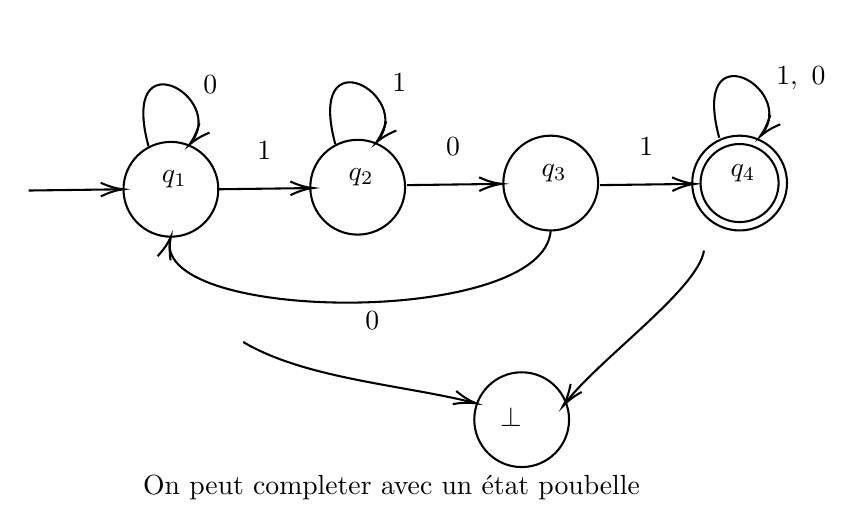
\begin{tikzpicture}[x=0.75pt,y=0.75pt,yscale=-1,xscale=1]
%uncomment if require: \path (0,300); %set diagram left start at 0, and has height of 300

%Shape: Circle [id:dp39159318436141544] 
\draw   (176,104.83) .. controls (176,92.22) and (186.22,82) .. (198.83,82) .. controls (211.44,82) and (221.67,92.22) .. (221.67,104.83) .. controls (221.67,117.44) and (211.44,127.67) .. (198.83,127.67) .. controls (186.22,127.67) and (176,117.44) .. (176,104.83) -- cycle ;
%Straight Lines [id:da23215206629411345] 
\draw    (130.33,105.43) -- (174,104.86) ;
\draw [shift={(176,104.83)}, rotate = 179.25] [color={rgb, 255:red, 0; green, 0; blue, 0 }  ][line width=0.75]    (10.93,-3.29) .. controls (6.95,-1.4) and (3.31,-0.3) .. (0,0) .. controls (3.31,0.3) and (6.95,1.4) .. (10.93,3.29)   ;
%Straight Lines [id:da6737208613248838] 
\draw    (221.67,104.83) -- (265.33,104.26) ;
\draw [shift={(267.33,104.23)}, rotate = 179.25] [color={rgb, 255:red, 0; green, 0; blue, 0 }  ][line width=0.75]    (10.93,-3.29) .. controls (6.95,-1.4) and (3.31,-0.3) .. (0,0) .. controls (3.31,0.3) and (6.95,1.4) .. (10.93,3.29)   ;
%Curve Lines [id:da7591834521750506] 
\draw    (188,84) .. controls (173.95,31.47) and (225.53,60.19) .. (208.78,82.07) ;
\draw [shift={(207.67,83.4)}, rotate = 312.27] [color={rgb, 255:red, 0; green, 0; blue, 0 }  ][line width=0.75]    (10.93,-3.29) .. controls (6.95,-1.4) and (3.31,-0.3) .. (0,0) .. controls (3.31,0.3) and (6.95,1.4) .. (10.93,3.29)   ;
%Shape: Circle [id:dp10471981573749756] 
\draw   (266,103.83) .. controls (266,91.22) and (276.22,81) .. (288.83,81) .. controls (301.44,81) and (311.67,91.22) .. (311.67,103.83) .. controls (311.67,116.44) and (301.44,126.67) .. (288.83,126.67) .. controls (276.22,126.67) and (266,116.44) .. (266,103.83) -- cycle ;
%Curve Lines [id:da770033043384433] 
\draw    (278,83) .. controls (263.95,30.47) and (315.53,59.19) .. (298.78,81.07) ;
\draw [shift={(297.67,82.4)}, rotate = 312.27] [color={rgb, 255:red, 0; green, 0; blue, 0 }  ][line width=0.75]    (10.93,-3.29) .. controls (6.95,-1.4) and (3.31,-0.3) .. (0,0) .. controls (3.31,0.3) and (6.95,1.4) .. (10.93,3.29)   ;
%Straight Lines [id:da8119244816386826] 
\draw    (312.67,102.83) -- (356.33,102.26) ;
\draw [shift={(358.33,102.23)}, rotate = 179.25] [color={rgb, 255:red, 0; green, 0; blue, 0 }  ][line width=0.75]    (10.93,-3.29) .. controls (6.95,-1.4) and (3.31,-0.3) .. (0,0) .. controls (3.31,0.3) and (6.95,1.4) .. (10.93,3.29)   ;
%Shape: Circle [id:dp9002917350521505] 
\draw   (359,101.83) .. controls (359,89.22) and (369.22,79) .. (381.83,79) .. controls (394.44,79) and (404.67,89.22) .. (404.67,101.83) .. controls (404.67,114.44) and (394.44,124.67) .. (381.83,124.67) .. controls (369.22,124.67) and (359,114.44) .. (359,101.83) -- cycle ;
%Curve Lines [id:da8427815305530494] 
\draw    (381.83,124.67) .. controls (378.88,170.96) and (191.42,169.46) .. (198.38,129.52) ;
\draw [shift={(198.83,127.67)}, rotate = 107.51] [color={rgb, 255:red, 0; green, 0; blue, 0 }  ][line width=0.75]    (10.93,-3.29) .. controls (6.95,-1.4) and (3.31,-0.3) .. (0,0) .. controls (3.31,0.3) and (6.95,1.4) .. (10.93,3.29)   ;
%Straight Lines [id:da9519294285068559] 
\draw    (405.67,102.83) -- (449.33,102.26) ;
\draw [shift={(451.33,102.23)}, rotate = 179.25] [color={rgb, 255:red, 0; green, 0; blue, 0 }  ][line width=0.75]    (10.93,-3.29) .. controls (6.95,-1.4) and (3.31,-0.3) .. (0,0) .. controls (3.31,0.3) and (6.95,1.4) .. (10.93,3.29)   ;
%Shape: Circle [id:dp11252058259290443] 
\draw   (450,101.83) .. controls (450,89.22) and (460.22,79) .. (472.83,79) .. controls (485.44,79) and (495.67,89.22) .. (495.67,101.83) .. controls (495.67,114.44) and (485.44,124.67) .. (472.83,124.67) .. controls (460.22,124.67) and (450,114.44) .. (450,101.83) -- cycle ;
%Curve Lines [id:da9970488655619414] 
\draw    (463,80) .. controls (448.95,27.47) and (500.53,56.19) .. (483.78,78.07) ;
\draw [shift={(482.67,79.4)}, rotate = 312.27] [color={rgb, 255:red, 0; green, 0; blue, 0 }  ][line width=0.75]    (10.93,-3.29) .. controls (6.95,-1.4) and (3.31,-0.3) .. (0,0) .. controls (3.31,0.3) and (6.95,1.4) .. (10.93,3.29)   ;
%Curve Lines [id:da05531269471522049] 
\draw    (455.67,134.4) .. controls (452.73,153.02) and (405.29,186.43) .. (388.65,208.09) ;
\draw [shift={(387.67,209.4)}, rotate = 305.95] [color={rgb, 255:red, 0; green, 0; blue, 0 }  ][line width=0.75]    (10.93,-3.29) .. controls (6.95,-1.4) and (3.31,-0.3) .. (0,0) .. controls (3.31,0.3) and (6.95,1.4) .. (10.93,3.29)   ;
%Curve Lines [id:da0594437607240863] 
\draw    (233.67,178.4) .. controls (263.22,196.13) and (312.17,199.31) .. (344.53,207.62) ;
\draw [shift={(346,208)}, rotate = 194.89] [color={rgb, 255:red, 0; green, 0; blue, 0 }  ][line width=0.75]    (10.93,-3.29) .. controls (6.95,-1.4) and (3.31,-0.3) .. (0,0) .. controls (3.31,0.3) and (6.95,1.4) .. (10.93,3.29)   ;
%Shape: Circle [id:dp45992039591403555] 
\draw   (345,215.83) .. controls (345,203.22) and (355.22,193) .. (367.83,193) .. controls (380.44,193) and (390.67,203.22) .. (390.67,215.83) .. controls (390.67,228.44) and (380.44,238.67) .. (367.83,238.67) .. controls (355.22,238.67) and (345,228.44) .. (345,215.83) -- cycle ;
%Shape: Circle [id:dp6241378939791583] 
\draw   (454.03,101.83) .. controls (454.03,91.45) and (462.45,83.03) .. (472.83,83.03) .. controls (483.22,83.03) and (491.63,91.45) .. (491.63,101.83) .. controls (491.63,112.22) and (483.22,120.63) .. (472.83,120.63) .. controls (462.45,120.63) and (454.03,112.22) .. (454.03,101.83) -- cycle ;

% Text Node
\draw (193,94.4) node [anchor=north west][inner sep=0.75pt]    {$q_{1}$};
% Text Node
\draw (213,48.4) node [anchor=north west][inner sep=0.75pt]    {$0$};
% Text Node
\draw (239,80.4) node [anchor=north west][inner sep=0.75pt]    {$1$};
% Text Node
\draw (283,93.4) node [anchor=north west][inner sep=0.75pt]    {$q_{2}$};
% Text Node
\draw (304,47.4) node [anchor=north west][inner sep=0.75pt]    {$1$};
% Text Node
\draw (330,78.4) node [anchor=north west][inner sep=0.75pt]    {$0$};
% Text Node
\draw (376,91.4) node [anchor=north west][inner sep=0.75pt]    {$q_{3}$};
% Text Node
\draw (291,162.4) node [anchor=north west][inner sep=0.75pt]    {$0$};
% Text Node
\draw (423,78.4) node [anchor=north west][inner sep=0.75pt]    {$1$};
% Text Node
\draw (467,91.4) node [anchor=north west][inner sep=0.75pt]    {$q_{4}$};
% Text Node
\draw (489,44.4) node [anchor=north west][inner sep=0.75pt]    {$1,\ 0$};
% Text Node
\draw (184,241) node [anchor=north west][inner sep=0.75pt]   [align=left] {On peut completer avec un état poubelle};
% Text Node
\draw (356,208.4) node [anchor=north west][inner sep=0.75pt]    {$\perp $};


\end{tikzpicture}


\end{centering}

On peut tester l'automate sur différents mots et vérifier si l'état final est $q_4$ qui est acceptant. Dans ce cas le mot appartiendra au langage de l'automate.

\begin{remarque}
On peut remarquer que $w_1= 11$ et $w_2= 0001$ finissent sur le même état et en fait on verra qu'ils peuvent être vus comme équivalent en terme de continuiation qu'on verra plus tard.
\end{remarque}

En fait, un automate est $\mathcal{L}(\mathcal{A})\subseteq \Sigma^*$ qui prend $w\in \Sigma^*$ et qui accepte si $w\in \mathcal{L}(\mathcal{A})$ et le rejette sinon.

A présent, formalisons les différents concepts que nous avons rencontré.
\begin{definition}[Automate fini déterministe (DFA)]
Voici des définitions plus formelles.
\begin{enumerate}

    \item On définit un mot comme une suite finie de lettres (symboles) sur un aplhabet (ensemble de symbole) $\Sigma$.
    \item Un langage $\mathcal{L}$ est un sous-ensemble de tous les mots $\mathcal{L} \subseteq \Sigma^*$
    \item Soient $\Sigma$ un alphabet, $Q$ un ensemble fini (d'état ), $q_0\in Q$ un état initial, $F\subseteq Q$ l'ensemble des états acceptant et $\delta: Q\times \Sigma \to Q$ une fonction dites de transition. On définit un automate comme un tuple  $$\mathcal{A}= (Q, \Sigma, \delta, q_0, F)$$
    \item On définit un Run pour $w=a_1\cdots a_n\in \Sigma^*$ comme un séquence d'états $$\rho=r_0r_1\cdots r_n$$ tel que $r_0=q_0$ et $\forall 1\leq i \leq n, r_i = \delta(r_{i-1},a_i)$
    \item On dit que $w$ est acceptant si $r_n \in F$. De plus, on pose 
    $$
    \mathcal{L}(\mathcal{A})= \{w\in \Sigma^* | w \text{ est accepté par } \mathcal{A}\} 
    $$
    \item Un automate est déterministe si pour chaque mot il existe un unique run.


\end{enumerate}

\end{definition}

\begin{exemple}
   Considérons le langage $\mathcal{L}= \{w\in \{0,1\}^* | \text{ le nombre de 1 est pair}\}$
\end{exemple}

\begin{centering}
    

\tikzset{every picture/.style={line width=0.75pt}} %set default line width to 0.75pt        

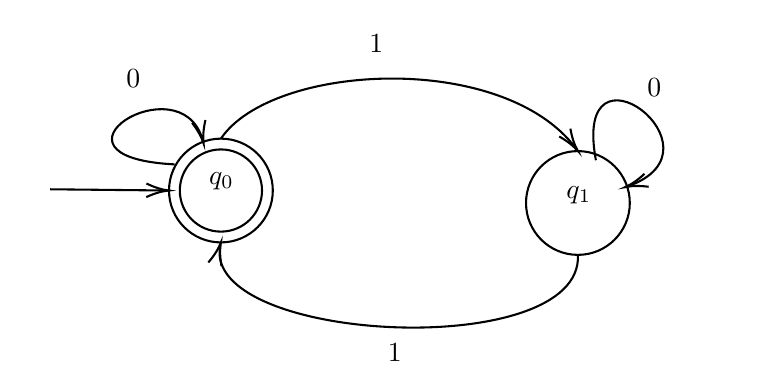
\begin{tikzpicture}[x=0.75pt,y=0.75pt,yscale=-1,xscale=1]
%uncomment if require: \path (0,300); %set diagram left start at 0, and has height of 300

%Shape: Circle [id:dp89135235634561] 
\draw   (168,132) .. controls (168,118.19) and (179.19,107) .. (193,107) .. controls (206.81,107) and (218,118.19) .. (218,132) .. controls (218,145.81) and (206.81,157) .. (193,157) .. controls (179.19,157) and (168,145.81) .. (168,132) -- cycle ;
%Shape: Circle [id:dp34115575534594467] 
\draw   (340,138) .. controls (340,124.19) and (351.19,113) .. (365,113) .. controls (378.81,113) and (390,124.19) .. (390,138) .. controls (390,151.81) and (378.81,163) .. (365,163) .. controls (351.19,163) and (340,151.81) .. (340,138) -- cycle ;
%Curve Lines [id:da7704822667159174] 
\draw    (193,107) .. controls (217.42,70.77) and (328.42,64.52) .. (363.95,111.56) ;
\draw [shift={(365,113)}, rotate = 234.76] [color={rgb, 255:red, 0; green, 0; blue, 0 }  ][line width=0.75]    (10.93,-3.29) .. controls (6.95,-1.4) and (3.31,-0.3) .. (0,0) .. controls (3.31,0.3) and (6.95,1.4) .. (10.93,3.29)   ;
%Curve Lines [id:da3551416469354568] 
\draw    (365,163) .. controls (367.64,214.88) and (183.41,205.59) .. (192.66,158.44) ;
\draw [shift={(193,157)}, rotate = 105.4] [color={rgb, 255:red, 0; green, 0; blue, 0 }  ][line width=0.75]    (10.93,-3.29) .. controls (6.95,-1.4) and (3.31,-0.3) .. (0,0) .. controls (3.31,0.3) and (6.95,1.4) .. (10.93,3.29)   ;
%Shape: Circle [id:dp11847089397851551] 
\draw   (173.2,132) .. controls (173.2,121.06) and (182.06,112.2) .. (193,112.2) .. controls (203.94,112.2) and (212.8,121.06) .. (212.8,132) .. controls (212.8,142.94) and (203.94,151.8) .. (193,151.8) .. controls (182.06,151.8) and (173.2,142.94) .. (173.2,132) -- cycle ;
%Curve Lines [id:da03166036311935516] 
\draw    (170.67,119.4) .. controls (100.4,115.85) and (173.41,69.81) .. (184.22,107.61) ;
\draw [shift={(184.67,109.4)}, rotate = 257.62] [color={rgb, 255:red, 0; green, 0; blue, 0 }  ][line width=0.75]    (10.93,-3.29) .. controls (6.95,-1.4) and (3.31,-0.3) .. (0,0) .. controls (3.31,0.3) and (6.95,1.4) .. (10.93,3.29)   ;
%Curve Lines [id:da48985526524398504] 
\draw    (373.67,117.4) .. controls (361.79,54.04) and (439.1,112.21) .. (389.22,129.88) ;
\draw [shift={(387.67,130.4)}, rotate = 342.22] [color={rgb, 255:red, 0; green, 0; blue, 0 }  ][line width=0.75]    (10.93,-3.29) .. controls (6.95,-1.4) and (3.31,-0.3) .. (0,0) .. controls (3.31,0.3) and (6.95,1.4) .. (10.93,3.29)   ;
%Straight Lines [id:da7792583689126359] 
\draw    (110.67,131.4) -- (166,131.98) ;
\draw [shift={(168,132)}, rotate = 180.6] [color={rgb, 255:red, 0; green, 0; blue, 0 }  ][line width=0.75]    (10.93,-3.29) .. controls (6.95,-1.4) and (3.31,-0.3) .. (0,0) .. controls (3.31,0.3) and (6.95,1.4) .. (10.93,3.29)   ;

% Text Node
\draw (185.8,121.8) node [anchor=north west][inner sep=0.75pt]    {$q_{0}$};
% Text Node
\draw (358,128.4) node [anchor=north west][inner sep=0.75pt]    {$q_{1}$};
% Text Node
\draw (272,204.4) node [anchor=north west][inner sep=0.75pt]    {$1$};
% Text Node
\draw (263,55.4) node [anchor=north west][inner sep=0.75pt]    {$1$};
% Text Node
\draw (146,72.4) node [anchor=north west][inner sep=0.75pt]    {$0$};
% Text Node
\draw (397,76.4) node [anchor=north west][inner sep=0.75pt]    {$0$};


\end{tikzpicture}

\end{centering}

\begin{exemple}
    pour $\mathcal{L}= \{w\in \{0,1\}^* | \text{ qui dit s'il y a autant de 0 que de 1 }\}$
    Il n'est pas possible de trouver un automate pour cela.
\end{exemple}

\section{Théorème de Klein}

Dans cette section, nous allons étudier le théorème de Kleen. Pour cette raison nous aurons besoins de différentes notions.

\begin{definition}[DFA-rec]
On dit qu'un langage $\mathcal{L}$ est reconnu par un DFA si il existe un automate qui accepte tous les mots du langage.
\end{definition}

\begin{theoreme}
Pour tout langage $\mathcal{L}$ on a l'équivalence entre $\mathcal{L}$ est reconnu par un $DFA$ et que $\mathcal{L}$ est défini par une RegExp. Si ces propositions sont vraies, on dit que $\mathcal{L}$ est régulier.
\end{theoreme}
 
\subsection{Expressions régulières}
Soient $\mathcal{L}_1$ et $\mathcal{L}_2$ deux langages sur un même alphabet (non nécéssaire), on définit :
\begin{itemize}
    \item $\mathcal{L}_1 \cup \mathcal{L}_2 = \{w | w\in \mathcal{L}_1 \lor w\in \mathcal{L}_2\} $
    \item $\mathcal{L}_1 \circ \mathcal{L}_2 = \{w_1w_2 | w_1\in \mathcal{L}_1 \land w_2\in \mathcal{L}_2  \}$
    \item $\mathcal{L}_1^*= \{w_1\dots w_k | k \geq 0 \land \forall 1\leq i \leq k, w_i \in \mathcal{L}_1\}$
\end{itemize}

\begin{exemple}
    Considérons $\mathcal{L}_1= \{\text{ Black, Yellow } \}$ et $\mathcal{L}_2= \{\text{ Night, Submarine }\}$
    \begin{itemize}
        \item $\mathcal{L}_1 \cup \mathcal{L}_2 = \{\text{ Black , Yellow , Night, Submarine }\}$
        \item $\mathcal{L}_1 \circ \mathcal{L}_2 = \{ \text{ BlackNight, BlackSubmarine, YellowNight, YellowSubmarine }\}$
        \item $ \mathcal{L}_1^*  =\{ \varepsilon, \text{ Black, Yellow, BlackYellow, ...} \} $
    \end{itemize}
\end{exemple}

Soit l'alphabet $\Sigma$ une expression régulière $E$ est formée de manière inductive par
$$E := \varnothing \, | \,\varepsilon \, | \, a \, | \, E+E' \, | \, EE' \quad  a \in \Sigma $$ 


\begin{exemple}
    Voici quelques exemples :
    \begin{itemize}
        \item $\mathcal{L}(\varnothing)= \varnothing$
        \item $\mathcal{L}(\varepsilon)= \{\varepsilon\}$
        \item $\mathcal{L}(E_1 +E_2 := E_1|E_2) = \mathcal{L}(E_1)\cup \mathcal{L}(E_2)$
        \item $\mathcal{L}(E_1E_2)= \mathcal{L}(E_1) \circ \mathcal{L}(E_2)$
        \item $\mathcal{L}(E^*)= \mathcal{L}(E)^*$
        \item $\mathcal{L}(E_1 \varnothing) = \varnothing$. 
        \item $\mathcal{L}(\varnothing^*)= \{\varepsilon\}$
        \item  Dés lors posons $\Sigma= \{a,b,c\}$
            \begin{itemize}
                \item $\mathcal{L}((a|b|c)^*)= \Sigma^*$
                \item $\mathcal{L}(a(b|c)^*a)= \{aba, aca ,abba , abca , acba, acca, \dots \}$
                \end{itemize}
    \end{itemize}

\end{exemple}

\begin{remarque}
    Ainsi le langage du premier automates est $\mathcal{L}(\mathcal{A})= \mathcal{L}((0|1)^* 101 (0|1)^*)$
\end{remarque}

Pour être clair, la \textbf{la priorité des opérations} est naturellement:

\begin{enumerate}
    \item $E^*$
    \item $EE'$
    \item $E+E'$
\end{enumerate}

Notons que le théorème de Kleen établit donc une équivalence entre deux objets qui pourtant semblent bien différents.
\subsection*{Regexp implique DFA}

Nous allons d'abord nous interesser à la direction RegExp implique DFA.
Pour cela, analysons d'abord \textbf{les propriétés de clôture} des langages reconnu par des DFA pour les opérations régulières.

\begin{lemme}
    Si $\mathcal{L}_1$ et  $\mathcal{L}_2$ sont des DFA-rec alors $\mathcal{L}_1 \cup \mathcal{L}_2$ est DFA-rec.
\end{lemme}

\begin{proof}
Débutons la preuve :  

Soient $\mathcal{A}_1= (Q_1, \Sigma, \delta_1, q_1, F_1)$ rec $\mathcal{L}_1$ et $\mathcal{A}_2= (Q_2, \Sigma, \delta_2, q_2, F_2)$ rec $\mathcal{L}_2$

Nous voulons construire $\mathcal{A}= (Q, \Sigma, \delta, q, F)$ tel que $\mathcal{L}(\mathcal{A}) = \mathcal{L}_1 \cup \mathcal{L}_2$.
Pour illustrer l'idée :

\bigskip


\tikzset{every picture/.style={line width=0.75pt}} %set default line width to 0.75pt        

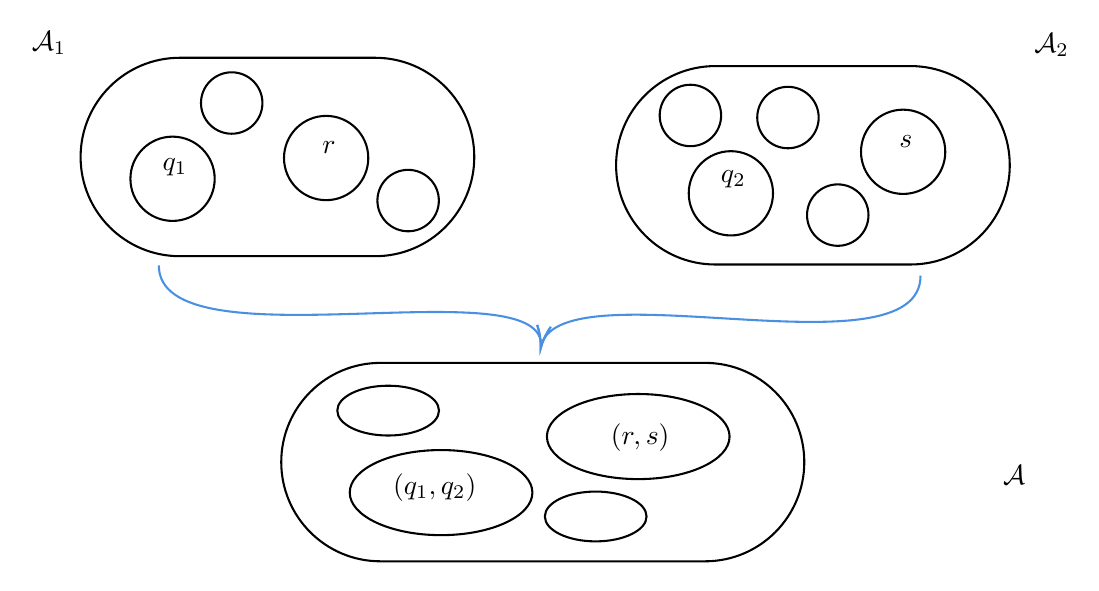
\begin{tikzpicture}[x=0.75pt,y=0.75pt,yscale=-1,xscale=1]
%uncomment if require: \path (0,300); %set diagram left start at 0, and has height of 300

%Rounded Rect [id:dp284850783195031] 
\draw   (105,84.2) .. controls (105,57.8) and (126.4,36.4) .. (152.8,36.4) -- (246.87,36.4) .. controls (273.27,36.4) and (294.67,57.8) .. (294.67,84.2) -- (294.67,84.2) .. controls (294.67,110.6) and (273.27,132) .. (246.87,132) -- (152.8,132) .. controls (126.4,132) and (105,110.6) .. (105,84.2) -- cycle ;
%Rounded Rect [id:dp276114117813971] 
\draw   (363,88.2) .. controls (363,61.8) and (384.4,40.4) .. (410.8,40.4) -- (504.87,40.4) .. controls (531.27,40.4) and (552.67,61.8) .. (552.67,88.2) -- (552.67,88.2) .. controls (552.67,114.6) and (531.27,136) .. (504.87,136) -- (410.8,136) .. controls (384.4,136) and (363,114.6) .. (363,88.2) -- cycle ;
%Rounded Rect [id:dp6256025734689729] 
\draw   (201.67,231.2) .. controls (201.67,204.8) and (223.07,183.4) .. (249.47,183.4) -- (405.87,183.4) .. controls (432.27,183.4) and (453.67,204.8) .. (453.67,231.2) -- (453.67,231.2) .. controls (453.67,257.6) and (432.27,279) .. (405.87,279) -- (249.47,279) .. controls (223.07,279) and (201.67,257.6) .. (201.67,231.2) -- cycle ;
%Curve Lines [id:da6632754137669762] 
\draw [color={rgb, 255:red, 74; green, 144; blue, 226 }  ,draw opacity=1 ]   (142.67,136.4) .. controls (142.67,185.65) and (327.01,136.91) .. (326.81,174.62) ;
\draw [shift={(326.67,176.4)}, rotate = 278.33] [color={rgb, 255:red, 74; green, 144; blue, 226 }  ,draw opacity=1 ][line width=0.75]    (10.93,-3.29) .. controls (6.95,-1.4) and (3.31,-0.3) .. (0,0) .. controls (3.31,0.3) and (6.95,1.4) .. (10.93,3.29)   ;
%Curve Lines [id:da29599343206949935] 
\draw [color={rgb, 255:red, 74; green, 144; blue, 226 }  ,draw opacity=1 ]   (509.67,141.4) .. controls (509.67,190.65) and (337.94,137.06) .. (327.05,174.62) ;
\draw [shift={(326.67,176.4)}, rotate = 278.33] [color={rgb, 255:red, 74; green, 144; blue, 226 }  ,draw opacity=1 ][line width=0.75]    (10.93,-3.29) .. controls (6.95,-1.4) and (3.31,-0.3) .. (0,0) .. controls (3.31,0.3) and (6.95,1.4) .. (10.93,3.29)   ;
%Shape: Circle [id:dp2291311830942766] 
\draw   (129,94.7) .. controls (129,83.49) and (138.09,74.4) .. (149.3,74.4) .. controls (160.51,74.4) and (169.6,83.49) .. (169.6,94.7) .. controls (169.6,105.91) and (160.51,115) .. (149.3,115) .. controls (138.09,115) and (129,105.91) .. (129,94.7) -- cycle ;
%Shape: Circle [id:dp749510468452781] 
\draw   (398,101.7) .. controls (398,90.49) and (407.09,81.4) .. (418.3,81.4) .. controls (429.51,81.4) and (438.6,90.49) .. (438.6,101.7) .. controls (438.6,112.91) and (429.51,122) .. (418.3,122) .. controls (407.09,122) and (398,112.91) .. (398,101.7) -- cycle ;
%Shape: Circle [id:dp8657139071930654] 
\draw   (203,84.7) .. controls (203,73.49) and (212.09,64.4) .. (223.3,64.4) .. controls (234.51,64.4) and (243.6,73.49) .. (243.6,84.7) .. controls (243.6,95.91) and (234.51,105) .. (223.3,105) .. controls (212.09,105) and (203,95.91) .. (203,84.7) -- cycle ;
%Shape: Circle [id:dp6192027417932944] 
\draw   (481,81.7) .. controls (481,70.49) and (490.09,61.4) .. (501.3,61.4) .. controls (512.51,61.4) and (521.6,70.49) .. (521.6,81.7) .. controls (521.6,92.91) and (512.51,102) .. (501.3,102) .. controls (490.09,102) and (481,92.91) .. (481,81.7) -- cycle ;
%Shape: Circle [id:dp061472703884228985] 
\draw   (163,58.2) .. controls (163,50.03) and (169.63,43.4) .. (177.8,43.4) .. controls (185.97,43.4) and (192.6,50.03) .. (192.6,58.2) .. controls (192.6,66.37) and (185.97,73) .. (177.8,73) .. controls (169.63,73) and (163,66.37) .. (163,58.2) -- cycle ;
%Shape: Circle [id:dp813206027399627] 
\draw   (248,105.2) .. controls (248,97.03) and (254.63,90.4) .. (262.8,90.4) .. controls (270.97,90.4) and (277.6,97.03) .. (277.6,105.2) .. controls (277.6,113.37) and (270.97,120) .. (262.8,120) .. controls (254.63,120) and (248,113.37) .. (248,105.2) -- cycle ;
%Shape: Circle [id:dp5214504256712712] 
\draw   (384,64.2) .. controls (384,56.03) and (390.63,49.4) .. (398.8,49.4) .. controls (406.97,49.4) and (413.6,56.03) .. (413.6,64.2) .. controls (413.6,72.37) and (406.97,79) .. (398.8,79) .. controls (390.63,79) and (384,72.37) .. (384,64.2) -- cycle ;
%Shape: Circle [id:dp1340813771933912] 
\draw   (455,112.2) .. controls (455,104.03) and (461.63,97.4) .. (469.8,97.4) .. controls (477.97,97.4) and (484.6,104.03) .. (484.6,112.2) .. controls (484.6,120.37) and (477.97,127) .. (469.8,127) .. controls (461.63,127) and (455,120.37) .. (455,112.2) -- cycle ;
%Shape: Circle [id:dp32750300866498583] 
\draw   (431,65.2) .. controls (431,57.03) and (437.63,50.4) .. (445.8,50.4) .. controls (453.97,50.4) and (460.6,57.03) .. (460.6,65.2) .. controls (460.6,73.37) and (453.97,80) .. (445.8,80) .. controls (437.63,80) and (431,73.37) .. (431,65.2) -- cycle ;
%Shape: Ellipse [id:dp11321520816783048] 
\draw   (234.67,245.9) .. controls (234.67,234.58) and (254.37,225.4) .. (278.67,225.4) .. controls (302.97,225.4) and (322.67,234.58) .. (322.67,245.9) .. controls (322.67,257.22) and (302.97,266.4) .. (278.67,266.4) .. controls (254.37,266.4) and (234.67,257.22) .. (234.67,245.9) -- cycle ;
%Shape: Ellipse [id:dp9205037378392791] 
\draw   (329.67,218.9) .. controls (329.67,207.58) and (349.37,198.4) .. (373.67,198.4) .. controls (397.97,198.4) and (417.67,207.58) .. (417.67,218.9) .. controls (417.67,230.22) and (397.97,239.4) .. (373.67,239.4) .. controls (349.37,239.4) and (329.67,230.22) .. (329.67,218.9) -- cycle ;
%Shape: Ellipse [id:dp10192943005563937] 
\draw   (228.67,206.4) .. controls (228.67,199.77) and (239.64,194.4) .. (253.17,194.4) .. controls (266.7,194.4) and (277.67,199.77) .. (277.67,206.4) .. controls (277.67,213.03) and (266.7,218.4) .. (253.17,218.4) .. controls (239.64,218.4) and (228.67,213.03) .. (228.67,206.4) -- cycle ;
%Shape: Ellipse [id:dp16203183907806462] 
\draw   (328.67,257.4) .. controls (328.67,250.77) and (339.64,245.4) .. (353.17,245.4) .. controls (366.7,245.4) and (377.67,250.77) .. (377.67,257.4) .. controls (377.67,264.03) and (366.7,269.4) .. (353.17,269.4) .. controls (339.64,269.4) and (328.67,264.03) .. (328.67,257.4) -- cycle ;

% Text Node
\draw (80,22.4) node [anchor=north west][inner sep=0.75pt]    {$\mathcal{A}_{1}$};
% Text Node
\draw (563,23.4) node [anchor=north west][inner sep=0.75pt]    {$\mathcal{A}_{2}$};
% Text Node
\draw (548,231.4) node [anchor=north west][inner sep=0.75pt]    {$\mathcal{A}$};
% Text Node
\draw (143,83.4) node [anchor=north west][inner sep=0.75pt]    {$q_{1}$};
% Text Node
\draw (412,89.4) node [anchor=north west][inner sep=0.75pt]    {$q_{2}$};
% Text Node
\draw (220,75.4) node [anchor=north west][inner sep=0.75pt]    {$r$};
% Text Node
\draw (498,72.4) node [anchor=north west][inner sep=0.75pt]    {$s$};
% Text Node
\draw (254.04,235.19) node [anchor=north west][inner sep=0.75pt]    {$( q_{1} ,q_{2})$};
% Text Node
\draw (359.04,211.19) node [anchor=north west][inner sep=0.75pt]    {$( r,s)$};


\end{tikzpicture}

\bigskip

Posons $Q= Q_1\times Q_2$ et $q_0 = \langle q_1,q_2 \rangle $ et $\delta(\langle r,s \rangle, a )= \langle \delta_1(r,a), \delta_2(s,a) \rangle $
Pour $F$ prendre $F_1 \times F_2$ ne convient pas. Cependant $F= (Q_1\times F_2) \cup (F_1 \times Q_2)$ convient car nous voulons que dés que un des deux langages acceptent un mot c'est accepté.
\bigskip
Pour s'en convaincre, Montrons que 
    \begin{itemize}
    \item$\mathcal{L}(\mathcal{A})\subseteq \mathcal(L)(\mathcal{A}_1)\cup \mathcal{L}(\mathcal{A}_2)$.

   Prenons un mot $w$ accepté par $\mathcal{A}$ ; on doit montrer qu'il est aussi
    accepté par $\mathcal{A}_1$ ou $\mathcal{A}_2$. Par définition de
    $w \in \mathcal{L}(\mathcal{A})$, le run de $w$ dans $\mathcal{A}$ s'arrête sur
    un état de $F$, c'est-à-dire un couple $\langle r, s \rangle$ tel que
    $r \in F_1$ ou $s \in F_2$. Sans perte de généralité, supposons que $r \in F_1$.
    Le run dans $\mathcal{A}$ projeté dans $\mathcal{A}_1$ est un run de
    $\mathcal{A}_1$ qui finit en $r \in F_1$. Donc $\mathcal{A}_1$ accepte $w$ et
    $w \in \mathcal{L}_1$. A fortiori, $w \in \mathcal{L}_1 \cup \mathcal{L}_2$.

    \item $\mathcal{L}_1 \cup \mathcal{L}_2 \subseteq \mathcal{L}(\mathcal{A})$.

    Prenons un mot $w$ accepté par $\mathcal{A}_1$ (sans perte de généralité).
    Son run dans $\mathcal{A}_1$ peut être reproduit dans $\mathcal{A}$ par
    construction, et finit dans un état $\langle r, s \rangle$ où $r \in F_1$
    (par hypothèse). Par définition de $F$, on a donc que $\mathcal{A}$ accepte
    aussi $w$, et $w \in \mathcal{L}(\mathcal{A})$.
    \end{itemize}

\end{proof}


\begin{lemme}[Clôture pour la concaténation]
    Si $\mathcal{L}_1$ et $\mathcal{L}_2$ sont deux langages DFA-rec alors $\mathcal{L}_1\circ \mathcal{L}_2$ est DFA-rec
\end{lemme}

Le lemme précédent semble compliqué à prouver (voir notes manuscrites pour plus de détails).
En effet, Il apparait que pour construire un tel objet nous aurions besoin de connaitre le "future" d'un mot.
Pour contourner ce problème nous allons, à présent, nous intéresser aux automates non déterministes.





\subsection{Automates non déterministes}
Abordons, d'abord, cette notion par un exemple.

\begin{exemple}[NFA epsilon]
    Posons $\Sigma = \{a,b\}$ considérons l'automate suivant :



\tikzset{every picture/.style={line width=0.75pt}} %set default line width to 0.75pt        

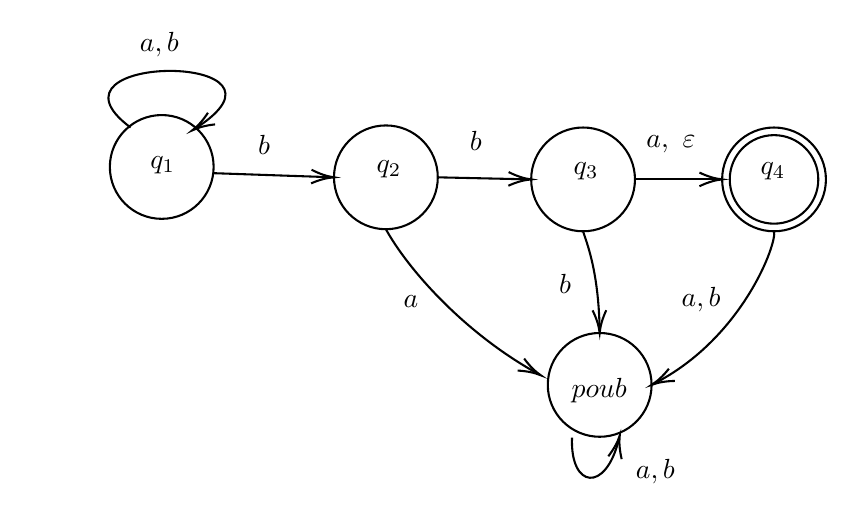
\begin{tikzpicture}[x=0.75pt,y=0.75pt,yscale=-1,xscale=1]
%uncomment if require: \path (0,300); %set diagram left start at 0, and has height of 300

%Shape: Circle [id:dp08765716097987719] 
\draw   (311,231) .. controls (311,217.19) and (322.19,206) .. (336,206) .. controls (349.81,206) and (361,217.19) .. (361,231) .. controls (361,244.81) and (349.81,256) .. (336,256) .. controls (322.19,256) and (311,244.81) .. (311,231) -- cycle ;
%Shape: Circle [id:dp3433082035661834] 
\draw   (208,131) .. controls (208,117.19) and (219.19,106) .. (233,106) .. controls (246.81,106) and (258,117.19) .. (258,131) .. controls (258,144.81) and (246.81,156) .. (233,156) .. controls (219.19,156) and (208,144.81) .. (208,131) -- cycle ;
%Shape: Circle [id:dp3347631803577762] 
\draw   (303,132) .. controls (303,118.19) and (314.19,107) .. (328,107) .. controls (341.81,107) and (353,118.19) .. (353,132) .. controls (353,145.81) and (341.81,157) .. (328,157) .. controls (314.19,157) and (303,145.81) .. (303,132) -- cycle ;
%Shape: Circle [id:dp8009869037853988] 
\draw   (395,132) .. controls (395,118.19) and (406.19,107) .. (420,107) .. controls (433.81,107) and (445,118.19) .. (445,132) .. controls (445,145.81) and (433.81,157) .. (420,157) .. controls (406.19,157) and (395,145.81) .. (395,132) -- cycle ;
%Curve Lines [id:da8950043269282352] 
\draw    (110,107) .. controls (60.91,70.58) and (200.26,70.4) .. (140.58,107.83) ;
\draw [shift={(139.67,108.4)}, rotate = 328.5] [color={rgb, 255:red, 0; green, 0; blue, 0 }  ][line width=0.75]    (10.93,-3.29) .. controls (6.95,-1.4) and (3.31,-0.3) .. (0,0) .. controls (3.31,0.3) and (6.95,1.4) .. (10.93,3.29)   ;
%Straight Lines [id:da2745951167254401] 
\draw    (150,129) -- (206,130.93) ;
\draw [shift={(208,131)}, rotate = 181.97] [color={rgb, 255:red, 0; green, 0; blue, 0 }  ][line width=0.75]    (10.93,-3.29) .. controls (6.95,-1.4) and (3.31,-0.3) .. (0,0) .. controls (3.31,0.3) and (6.95,1.4) .. (10.93,3.29)   ;
%Straight Lines [id:da9580631275356766] 
\draw    (258,131) -- (301,131.96) ;
\draw [shift={(303,132)}, rotate = 181.27] [color={rgb, 255:red, 0; green, 0; blue, 0 }  ][line width=0.75]    (10.93,-3.29) .. controls (6.95,-1.4) and (3.31,-0.3) .. (0,0) .. controls (3.31,0.3) and (6.95,1.4) .. (10.93,3.29)   ;
%Straight Lines [id:da08401375659539545] 
\draw    (353,132) -- (393,132) ;
\draw [shift={(395,132)}, rotate = 180] [color={rgb, 255:red, 0; green, 0; blue, 0 }  ][line width=0.75]    (10.93,-3.29) .. controls (6.95,-1.4) and (3.31,-0.3) .. (0,0) .. controls (3.31,0.3) and (6.95,1.4) .. (10.93,3.29)   ;
%Shape: Circle [id:dp6497837056980355] 
\draw   (398.67,132) .. controls (398.67,120.22) and (408.22,110.67) .. (420,110.67) .. controls (431.78,110.67) and (441.33,120.22) .. (441.33,132) .. controls (441.33,143.78) and (431.78,153.33) .. (420,153.33) .. controls (408.22,153.33) and (398.67,143.78) .. (398.67,132) -- cycle ;
%Shape: Circle [id:dp9063178066043676] 
\draw   (100,126) .. controls (100,112.19) and (111.19,101) .. (125,101) .. controls (138.81,101) and (150,112.19) .. (150,126) .. controls (150,139.81) and (138.81,151) .. (125,151) .. controls (111.19,151) and (100,139.81) .. (100,126) -- cycle ;
%Curve Lines [id:da7888681322676493] 
\draw    (233,156) .. controls (243.51,175.11) and (270.51,205.86) .. (306.04,225.51) ;
\draw [shift={(307.67,226.4)}, rotate = 208.34] [color={rgb, 255:red, 0; green, 0; blue, 0 }  ][line width=0.75]    (10.93,-3.29) .. controls (6.95,-1.4) and (3.31,-0.3) .. (0,0) .. controls (3.31,0.3) and (6.95,1.4) .. (10.93,3.29)   ;
%Curve Lines [id:da5598456428758242] 
\draw    (328,157) .. controls (329.63,162.29) and (335.43,175.84) .. (335.97,204.24) ;
\draw [shift={(336,206)}, rotate = 269.35] [color={rgb, 255:red, 0; green, 0; blue, 0 }  ][line width=0.75]    (10.93,-3.29) .. controls (6.95,-1.4) and (3.31,-0.3) .. (0,0) .. controls (3.31,0.3) and (6.95,1.4) .. (10.93,3.29)   ;
%Curve Lines [id:da8995112956133697] 
\draw    (420,157) .. controls (421.65,162.35) and (405,208.46) .. (362.3,230.34) ;
\draw [shift={(361,231)}, rotate = 333.68] [color={rgb, 255:red, 0; green, 0; blue, 0 }  ][line width=0.75]    (10.93,-3.29) .. controls (6.95,-1.4) and (3.31,-0.3) .. (0,0) .. controls (3.31,0.3) and (6.95,1.4) .. (10.93,3.29)   ;
%Curve Lines [id:da6651337017429059] 
\draw    (322.67,256.4) .. controls (321.69,280.9) and (338.95,283.31) .. (345.29,257.04) ;
\draw [shift={(345.67,255.4)}, rotate = 102.09] [color={rgb, 255:red, 0; green, 0; blue, 0 }  ][line width=0.75]    (10.93,-3.29) .. controls (6.95,-1.4) and (3.31,-0.3) .. (0,0) .. controls (3.31,0.3) and (6.95,1.4) .. (10.93,3.29)   ;

% Text Node
\draw (113,59.4) node [anchor=north west][inner sep=0.75pt]    {$a,b$};
% Text Node
\draw (118,119.4) node [anchor=north west][inner sep=0.75pt]    {$q_{1}$};
% Text Node
\draw (322,122.4) node [anchor=north west][inner sep=0.75pt]    {$q_{3}$};
% Text Node
\draw (227,121.4) node [anchor=north west][inner sep=0.75pt]    {$q_{2}$};
% Text Node
\draw (412,122.4) node [anchor=north west][inner sep=0.75pt]    {$q_{4}$};
% Text Node
\draw (170,109.4) node [anchor=north west][inner sep=0.75pt]    {$b$};
% Text Node
\draw (272,107.4) node [anchor=north west][inner sep=0.75pt]    {$b$};
% Text Node
\draw (357,109.4) node [anchor=north west][inner sep=0.75pt]    {$a,\ \varepsilon $};
% Text Node
\draw (240,186.4) node [anchor=north west][inner sep=0.75pt]    {$a$};
% Text Node
\draw (315,176.4) node [anchor=north west][inner sep=0.75pt]    {$b$};
% Text Node
\draw (374,182.4) node [anchor=north west][inner sep=0.75pt]    {$a,b$};
% Text Node
\draw (352,265.4) node [anchor=north west][inner sep=0.75pt]    {$a,b$};
% Text Node
\draw (321,226.4) node [anchor=north west][inner sep=0.75pt]    {$poub$};


\end{tikzpicture}

Dans ce cas, il y a plusieurs runs par mot s'il existe une run où le mot est accepté alors le mot est accepté et que tout le mot soit lu.
Par exemple avec le mot $w = abba $ ca donne : 

\bigskip

\tikzset{every picture/.style={line width=0.75pt}} %set default line width to 0.75pt        
\begin{centering}
    

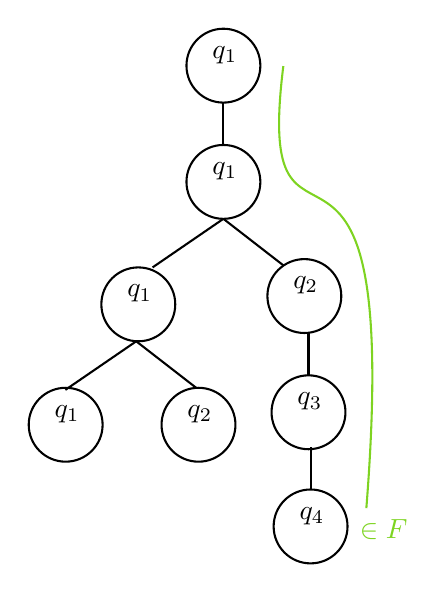
\begin{tikzpicture}[x=0.75pt,y=0.75pt,yscale=-1,xscale=1]
%uncomment if require: \path (0,300); %set diagram left start at 0, and has height of 300

%Shape: Circle [id:dp6836294885390309] 
\draw   (303,53.2) .. controls (303,43.37) and (310.97,35.4) .. (320.8,35.4) .. controls (330.63,35.4) and (338.6,43.37) .. (338.6,53.2) .. controls (338.6,63.03) and (330.63,71) .. (320.8,71) .. controls (310.97,71) and (303,63.03) .. (303,53.2) -- cycle ;
%Straight Lines [id:da1797130402663174] 
\draw    (320.8,71) -- (320.8,91.4) ;
%Shape: Circle [id:dp3360194582447127] 
\draw   (303,109.2) .. controls (303,99.37) and (310.97,91.4) .. (320.8,91.4) .. controls (330.63,91.4) and (338.6,99.37) .. (338.6,109.2) .. controls (338.6,119.03) and (330.63,127) .. (320.8,127) .. controls (310.97,127) and (303,119.03) .. (303,109.2) -- cycle ;
%Straight Lines [id:da5468002279918187] 
\draw    (320.8,127) -- (286.67,150.4) ;
%Straight Lines [id:da5929348448495171] 
\draw    (320.8,127) -- (349.67,149.4) ;
%Shape: Circle [id:dp09070174132722919] 
\draw   (262,168.2) .. controls (262,158.37) and (269.97,150.4) .. (279.8,150.4) .. controls (289.63,150.4) and (297.6,158.37) .. (297.6,168.2) .. controls (297.6,178.03) and (289.63,186) .. (279.8,186) .. controls (269.97,186) and (262,178.03) .. (262,168.2) -- cycle ;
%Straight Lines [id:da7432525559126064] 
\draw    (278.8,186) -- (244.67,209.4) ;
%Straight Lines [id:da7092417830658024] 
\draw    (278.8,186) -- (307.67,208.4) ;
%Shape: Circle [id:dp3089281106642574] 
\draw   (227,226.2) .. controls (227,216.37) and (234.97,208.4) .. (244.8,208.4) .. controls (254.63,208.4) and (262.6,216.37) .. (262.6,226.2) .. controls (262.6,236.03) and (254.63,244) .. (244.8,244) .. controls (234.97,244) and (227,236.03) .. (227,226.2) -- cycle ;
%Shape: Circle [id:dp5878232654443346] 
\draw   (291,226.2) .. controls (291,216.37) and (298.97,208.4) .. (308.8,208.4) .. controls (318.63,208.4) and (326.6,216.37) .. (326.6,226.2) .. controls (326.6,236.03) and (318.63,244) .. (308.8,244) .. controls (298.97,244) and (291,236.03) .. (291,226.2) -- cycle ;
%Shape: Circle [id:dp9695784397920547] 
\draw   (342,164.2) .. controls (342,154.37) and (349.97,146.4) .. (359.8,146.4) .. controls (369.63,146.4) and (377.6,154.37) .. (377.6,164.2) .. controls (377.6,174.03) and (369.63,182) .. (359.8,182) .. controls (349.97,182) and (342,174.03) .. (342,164.2) -- cycle ;
%Straight Lines [id:da3460956435531176] 
\draw    (361.8,182) -- (361.8,202.4) ;
%Shape: Circle [id:dp383956515725579] 
\draw   (344,220.2) .. controls (344,210.37) and (351.97,202.4) .. (361.8,202.4) .. controls (371.63,202.4) and (379.6,210.37) .. (379.6,220.2) .. controls (379.6,230.03) and (371.63,238) .. (361.8,238) .. controls (351.97,238) and (344,230.03) .. (344,220.2) -- cycle ;
%Straight Lines [id:da3915738052577249] 
\draw    (362.8,237) -- (362.8,257.4) ;
%Shape: Circle [id:dp826651689011283] 
\draw   (345,275.2) .. controls (345,265.37) and (352.97,257.4) .. (362.8,257.4) .. controls (372.63,257.4) and (380.6,265.37) .. (380.6,275.2) .. controls (380.6,285.03) and (372.63,293) .. (362.8,293) .. controls (352.97,293) and (345,285.03) .. (345,275.2) -- cycle ;
%Curve Lines [id:da5610764930802694] 
\draw [color={rgb, 255:red, 126; green, 211; blue, 33 }  ,draw opacity=1 ]   (349.67,53.4) .. controls (334.67,173.4) and (407.67,38.4) .. (389.67,266.4) ;

% Text Node
\draw (314,42.4) node [anchor=north west][inner sep=0.75pt]    {$q_{1}$};
% Text Node
\draw (314,98.4) node [anchor=north west][inner sep=0.75pt]    {$q_{1}$};
% Text Node
\draw (273,157.4) node [anchor=north west][inner sep=0.75pt]    {$q_{1}$};
% Text Node
\draw (238,215.4) node [anchor=north west][inner sep=0.75pt]    {$q_{1}$};
% Text Node
\draw (302,215.4) node [anchor=north west][inner sep=0.75pt]    {$q_{2}$};
% Text Node
\draw (353,153.4) node [anchor=north west][inner sep=0.75pt]    {$q_{2}$};
% Text Node
\draw (355,209.4) node [anchor=north west][inner sep=0.75pt]    {$q_{3}$};
% Text Node
\draw (356,264.4) node [anchor=north west][inner sep=0.75pt]    {$q_{4}$};
% Text Node
\draw (385,270.4) node [anchor=north west][inner sep=0.75pt]    {$\textcolor[rgb]{0.49,0.83,0.13}{\in F}$};


\end{tikzpicture}

\end{centering}
Notons que $\mathcal{L}(\mathcal{A})= \mathcal{L}((a|b)^*bb(a|\varepsilon))$
\end{exemple}

Définissons formellement les NFA$\varepsilon$:

\begin{definition}[Automate fini non-déterministe avec $\varepsilon$-transitions]
Un NFA$\varepsilon$ est un tuple $\mathcal{A} = (Q, \Sigma, \delta, q_0, F)$ où
\begin{itemize}
    \item $Q$ est un ensemble fini d'états,
    \item $\Sigma$ est un alphabet fini,
    \item $q_0 \in Q$ est l'état initial,
    \item $F \subseteq Q$ est un ensemble d'états acceptants,
    \item $\delta : Q \times \Sigma_\varepsilon \to 2^Q$ est la fonction de transition.
\end{itemize}
\end{definition}

\begin{definition}[Run dans un NFA$\varepsilon$]
Un run pour un mot $w \in \Sigma^*$ est une séquence d'états
$\rho = r_0 \cdots r_m$ associée à une séquence de symboles
$a_1 \cdots a_m \in \Sigma_\varepsilon^*$ telle que
\begin{itemize}
    \item $r_0 = q_0$,
    \item $\forall 1 \leq i \leq m,\ r_i \in \delta(r_{i-1}, a_i)$,
    \item $w = a_1 \cdot a_2 \cdots a_m$.
\end{itemize}
\end{definition}

\begin{definition}[Acceptance dans un NFA$\varepsilon$]
Un mot $w$ est accepté s'il existe un run $\rho = r_0 \cdots r_m$ sur ce mot
tel que $r_m \in F$.
\end{definition}

\paragraph{Trois visions du non-déterminisme}

\begin{enumerate}
    \item \textbf{arbres.}
    Nous créons un arbre d'exécution avec un branchement pour chaque choix
    non-déterministe : nous acceptons si une des branches accepte.

    \item \textbf{calcul parallèle.}
    À chaque choix non-déterministe, nous faisons un \og fork \fg{} : nous lançons
    un nouveau processus qui fonctionne en parallèle. Nous acceptons si un des
    processus accepte.

    \item \textbf{Magique}
    Nous \og devinons \fg{} le choix correct (celui qui amènera à OUI) et nous
    allons de ce côté.
\end{enumerate}

\begin{proposition}
    On peut transformer tout NFA$\varepsilon$ $\mathcal{A}_\varepsilon$ en NFA (sans $\varepsilon$ transition) $\mathcal{A}$ équivalent. Autrement dit,
    $$\mathcal{L}(\mathcal{A}_\varepsilon)=\mathcal{L}(\mathcal{A})$$
\end{proposition}

\begin{proof}
    
\end{proof}

\begin{theoreme}
Pour tout NFA $\mathcal{A}$, il existe un DFA $\mathcal{A}'$ tel que
    $$\mathcal{L}(\mathcal{A}) = \mathcal{L}(\mathcal{A}')$$
\end{theoreme}

\begin{proof}
    Soit $\mathcal{A} = (Q, \Sigma, \delta, q_0, F)$ un NFA. Nous allons construire un DFA $\mathcal{A}' = (Q', \Sigma, \delta', q_0', F')$ tel que $Q' = 2^Q$ et $\delta'(R,a) = \{q \in Q \mid \exists r \in R, q \in \delta(r,a)\}$. 
\end{proof}


\begin{exemple}

    Considérons le NFA suivant :
\begin{center}


\tikzset{every picture/.style={line width=0.75pt}} %set default line width to 0.75pt        

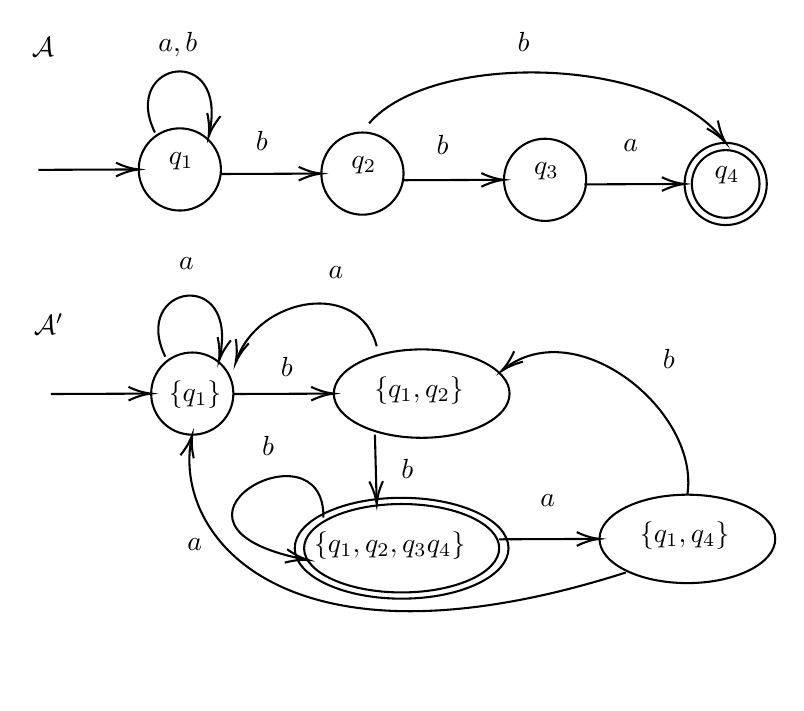
\begin{tikzpicture}[x=0.75pt,y=0.75pt,yscale=-1,xscale=1]
%uncomment if require: \path (0,300); %set diagram left start at 0, and has height of 300

%Shape: Circle [id:dp7103996276945939] 
\draw   (194,72.2) .. controls (194,61.26) and (202.86,52.4) .. (213.8,52.4) .. controls (224.74,52.4) and (233.6,61.26) .. (233.6,72.2) .. controls (233.6,83.14) and (224.74,92) .. (213.8,92) .. controls (202.86,92) and (194,83.14) .. (194,72.2) -- cycle ;
%Straight Lines [id:da6059613049447466] 
\draw    (145.67,72.4) -- (192,72.21) ;
\draw [shift={(194,72.2)}, rotate = 179.76] [color={rgb, 255:red, 0; green, 0; blue, 0 }  ][line width=0.75]    (10.93,-3.29) .. controls (6.95,-1.4) and (3.31,-0.3) .. (0,0) .. controls (3.31,0.3) and (6.95,1.4) .. (10.93,3.29)   ;
%Shape: Circle [id:dp026295764448947545] 
\draw   (282,74.2) .. controls (282,63.26) and (290.86,54.4) .. (301.8,54.4) .. controls (312.74,54.4) and (321.6,63.26) .. (321.6,74.2) .. controls (321.6,85.14) and (312.74,94) .. (301.8,94) .. controls (290.86,94) and (282,85.14) .. (282,74.2) -- cycle ;
%Straight Lines [id:da4196285531589641] 
\draw    (233.67,74.4) -- (280,74.21) ;
\draw [shift={(282,74.2)}, rotate = 179.76] [color={rgb, 255:red, 0; green, 0; blue, 0 }  ][line width=0.75]    (10.93,-3.29) .. controls (6.95,-1.4) and (3.31,-0.3) .. (0,0) .. controls (3.31,0.3) and (6.95,1.4) .. (10.93,3.29)   ;
%Shape: Circle [id:dp8333435694396505] 
\draw   (370,77.2) .. controls (370,66.26) and (378.86,57.4) .. (389.8,57.4) .. controls (400.74,57.4) and (409.6,66.26) .. (409.6,77.2) .. controls (409.6,88.14) and (400.74,97) .. (389.8,97) .. controls (378.86,97) and (370,88.14) .. (370,77.2) -- cycle ;
%Straight Lines [id:da8666297176116446] 
\draw    (321.67,77.4) -- (368,77.21) ;
\draw [shift={(370,77.2)}, rotate = 179.76] [color={rgb, 255:red, 0; green, 0; blue, 0 }  ][line width=0.75]    (10.93,-3.29) .. controls (6.95,-1.4) and (3.31,-0.3) .. (0,0) .. controls (3.31,0.3) and (6.95,1.4) .. (10.93,3.29)   ;
%Shape: Circle [id:dp7499527940101318] 
\draw   (457,79.2) .. controls (457,68.26) and (465.86,59.4) .. (476.8,59.4) .. controls (487.74,59.4) and (496.6,68.26) .. (496.6,79.2) .. controls (496.6,90.14) and (487.74,99) .. (476.8,99) .. controls (465.86,99) and (457,90.14) .. (457,79.2) -- cycle ;
%Straight Lines [id:da1959703394632939] 
\draw    (408.67,79.4) -- (455,79.21) ;
\draw [shift={(457,79.2)}, rotate = 179.76] [color={rgb, 255:red, 0; green, 0; blue, 0 }  ][line width=0.75]    (10.93,-3.29) .. controls (6.95,-1.4) and (3.31,-0.3) .. (0,0) .. controls (3.31,0.3) and (6.95,1.4) .. (10.93,3.29)   ;
%Curve Lines [id:da6667632608657935] 
\draw    (305,50) .. controls (334.37,15.75) and (443.45,16.38) .. (475.84,58.12) ;
\draw [shift={(476.8,59.4)}, rotate = 234.09] [color={rgb, 255:red, 0; green, 0; blue, 0 }  ][line width=0.75]    (10.93,-3.29) .. controls (6.95,-1.4) and (3.31,-0.3) .. (0,0) .. controls (3.31,0.3) and (6.95,1.4) .. (10.93,3.29)   ;
%Curve Lines [id:da6933603849222757] 
\draw    (201.8,54.4) .. controls (184.84,19.75) and (237.59,10.58) .. (227.98,55.04) ;
\draw [shift={(227.67,56.4)}, rotate = 283.45] [color={rgb, 255:red, 0; green, 0; blue, 0 }  ][line width=0.75]    (10.93,-3.29) .. controls (6.95,-1.4) and (3.31,-0.3) .. (0,0) .. controls (3.31,0.3) and (6.95,1.4) .. (10.93,3.29)   ;
%Shape: Circle [id:dp2235202354194894] 
\draw   (460.5,79.2) .. controls (460.5,70.2) and (467.8,62.9) .. (476.8,62.9) .. controls (485.8,62.9) and (493.1,70.2) .. (493.1,79.2) .. controls (493.1,88.2) and (485.8,95.5) .. (476.8,95.5) .. controls (467.8,95.5) and (460.5,88.2) .. (460.5,79.2) -- cycle ;
%Shape: Circle [id:dp37306961721295884] 
\draw   (200,180.2) .. controls (200,169.26) and (208.86,160.4) .. (219.8,160.4) .. controls (230.74,160.4) and (239.6,169.26) .. (239.6,180.2) .. controls (239.6,191.14) and (230.74,200) .. (219.8,200) .. controls (208.86,200) and (200,191.14) .. (200,180.2) -- cycle ;
%Straight Lines [id:da4799886521048061] 
\draw    (151.67,180.4) -- (198,180.21) ;
\draw [shift={(200,180.2)}, rotate = 179.76] [color={rgb, 255:red, 0; green, 0; blue, 0 }  ][line width=0.75]    (10.93,-3.29) .. controls (6.95,-1.4) and (3.31,-0.3) .. (0,0) .. controls (3.31,0.3) and (6.95,1.4) .. (10.93,3.29)   ;
%Curve Lines [id:da5158343722294488] 
\draw    (206.8,162.4) .. controls (189.84,127.75) and (242.59,118.58) .. (232.98,163.04) ;
\draw [shift={(232.67,164.4)}, rotate = 283.45] [color={rgb, 255:red, 0; green, 0; blue, 0 }  ][line width=0.75]    (10.93,-3.29) .. controls (6.95,-1.4) and (3.31,-0.3) .. (0,0) .. controls (3.31,0.3) and (6.95,1.4) .. (10.93,3.29)   ;
%Straight Lines [id:da1375078792035651] 
\draw    (239.67,180.4) -- (286,180.21) ;
\draw [shift={(288,180.2)}, rotate = 179.76] [color={rgb, 255:red, 0; green, 0; blue, 0 }  ][line width=0.75]    (10.93,-3.29) .. controls (6.95,-1.4) and (3.31,-0.3) .. (0,0) .. controls (3.31,0.3) and (6.95,1.4) .. (10.93,3.29)   ;
%Straight Lines [id:da7501785526978499] 
\draw    (307.8,200) -- (308.61,231.4) ;
\draw [shift={(308.67,233.4)}, rotate = 268.51] [color={rgb, 255:red, 0; green, 0; blue, 0 }  ][line width=0.75]    (10.93,-3.29) .. controls (6.95,-1.4) and (3.31,-0.3) .. (0,0) .. controls (3.31,0.3) and (6.95,1.4) .. (10.93,3.29)   ;
%Shape: Ellipse [id:dp41161783164005084] 
\draw   (273.67,254.7) .. controls (273.67,242.94) and (294.71,233.4) .. (320.67,233.4) .. controls (346.62,233.4) and (367.67,242.94) .. (367.67,254.7) .. controls (367.67,266.46) and (346.62,276) .. (320.67,276) .. controls (294.71,276) and (273.67,266.46) .. (273.67,254.7) -- cycle ;
%Straight Lines [id:da7523391329347832] 
\draw    (367.67,250.4) -- (414,250.21) ;
\draw [shift={(416,250.2)}, rotate = 179.76] [color={rgb, 255:red, 0; green, 0; blue, 0 }  ][line width=0.75]    (10.93,-3.29) .. controls (6.95,-1.4) and (3.31,-0.3) .. (0,0) .. controls (3.31,0.3) and (6.95,1.4) .. (10.93,3.29)   ;
%Curve Lines [id:da6096081426059904] 
\draw    (428.67,266.4) .. controls (264.33,318.87) and (209.76,248.83) .. (219.49,201.43) ;
\draw [shift={(219.8,200)}, rotate = 103.22] [color={rgb, 255:red, 0; green, 0; blue, 0 }  ][line width=0.75]    (10.93,-3.29) .. controls (6.95,-1.4) and (3.31,-0.3) .. (0,0) .. controls (3.31,0.3) and (6.95,1.4) .. (10.93,3.29)   ;
%Curve Lines [id:da27484747173679214] 
\draw    (283,240) .. controls (283.66,191.64) and (189.61,243.87) .. (274.38,260.16) ;
\draw [shift={(275.67,260.4)}, rotate = 190.42] [color={rgb, 255:red, 0; green, 0; blue, 0 }  ][line width=0.75]    (10.93,-3.29) .. controls (6.95,-1.4) and (3.31,-0.3) .. (0,0) .. controls (3.31,0.3) and (6.95,1.4) .. (10.93,3.29)   ;
%Curve Lines [id:da3042426824548118] 
\draw    (308.67,157.4) .. controls (300.46,125.29) and (252.15,133.15) .. (241.14,163.98) ;
\draw [shift={(240.67,165.4)}, rotate = 287.35] [color={rgb, 255:red, 0; green, 0; blue, 0 }  ][line width=0.75]    (10.93,-3.29) .. controls (6.95,-1.4) and (3.31,-0.3) .. (0,0) .. controls (3.31,0.3) and (6.95,1.4) .. (10.93,3.29)   ;
%Curve Lines [id:da3244162208609642] 
\draw    (458.33,228.9) .. controls (464.6,188.8) and (404.95,140.58) .. (369.73,168.53) ;
\draw [shift={(368.67,169.4)}, rotate = 319.64] [color={rgb, 255:red, 0; green, 0; blue, 0 }  ][line width=0.75]    (10.93,-3.29) .. controls (6.95,-1.4) and (3.31,-0.3) .. (0,0) .. controls (3.31,0.3) and (6.95,1.4) .. (10.93,3.29)   ;
%Shape: Ellipse [id:dp9197986403833979] 
\draw   (288,180.2) .. controls (288,168.44) and (306.95,158.9) .. (330.33,158.9) .. controls (353.71,158.9) and (372.67,168.44) .. (372.67,180.2) .. controls (372.67,191.96) and (353.71,201.5) .. (330.33,201.5) .. controls (306.95,201.5) and (288,191.96) .. (288,180.2) -- cycle ;
%Shape: Ellipse [id:dp024258727052963724] 
\draw   (416,250.2) .. controls (416,238.44) and (434.95,228.9) .. (458.33,228.9) .. controls (481.71,228.9) and (500.67,238.44) .. (500.67,250.2) .. controls (500.67,261.96) and (481.71,271.5) .. (458.33,271.5) .. controls (434.95,271.5) and (416,261.96) .. (416,250.2) -- cycle ;
%Shape: Ellipse [id:dp2401172975401179] 
\draw   (269.17,254.7) .. controls (269.17,241.28) and (292.22,230.4) .. (320.67,230.4) .. controls (349.11,230.4) and (372.17,241.28) .. (372.17,254.7) .. controls (372.17,268.12) and (349.11,279) .. (320.67,279) .. controls (292.22,279) and (269.17,268.12) .. (269.17,254.7) -- cycle ;

% Text Node
\draw (207,62.4) node [anchor=north west][inner sep=0.75pt]    {$q_{1}$};
% Text Node
\draw (295,64.4) node [anchor=north west][inner sep=0.75pt]    {$q_{2}$};
% Text Node
\draw (383,67.4) node [anchor=north west][inner sep=0.75pt]    {$q_{3}$};
% Text Node
\draw (470,69.4) node [anchor=north west][inner sep=0.75pt]    {$q_{4}$};
% Text Node
\draw (141,7.4) node [anchor=north west][inner sep=0.75pt]    {$\mathcal{A}$};
% Text Node
\draw (202,4.4) node [anchor=north west][inner sep=0.75pt]    {$a,b$};
% Text Node
\draw (249,52.4) node [anchor=north west][inner sep=0.75pt]    {$b$};
% Text Node
\draw (336,54.4) node [anchor=north west][inner sep=0.75pt]    {$b$};
% Text Node
\draw (375,4.4) node [anchor=north west][inner sep=0.75pt]    {$b$};
% Text Node
\draw (426,56.4) node [anchor=north west][inner sep=0.75pt]    {$a$};
% Text Node
\draw (142,140.4) node [anchor=north west][inner sep=0.75pt]    {$\mathcal{A} '$};
% Text Node
\draw (306,170.4) node [anchor=north west][inner sep=0.75pt]    {$\{q_{1} ,q_{2}\}$};
% Text Node
\draw (277,245.4) node [anchor=north west][inner sep=0.75pt]    {$\{q_{1} ,q_{2} ,q_{3} q_{4}\}$};
% Text Node
\draw (434,240.4) node [anchor=north west][inner sep=0.75pt]    {$\{q_{1} ,q_{4}\}$};
% Text Node
\draw (207,172.4) node [anchor=north west][inner sep=0.75pt]    {$\{q_{1}\}$};
% Text Node
\draw (386,227.4) node [anchor=north west][inner sep=0.75pt]    {$a$};
% Text Node
\draw (319,210.4) node [anchor=north west][inner sep=0.75pt]    {$b$};
% Text Node
\draw (445,157.4) node [anchor=north west][inner sep=0.75pt]    {$b$};
% Text Node
\draw (261,161.4) node [anchor=north west][inner sep=0.75pt]    {$b$};
% Text Node
\draw (252,199.4) node [anchor=north west][inner sep=0.75pt]    {$b$};
% Text Node
\draw (212,113.4) node [anchor=north west][inner sep=0.75pt]    {$a$};
% Text Node
\draw (284,117.4) node [anchor=north west][inner sep=0.75pt]    {$a$};
% Text Node
\draw (216,248.4) node [anchor=north west][inner sep=0.75pt]    {$a$};


\end{tikzpicture}

\end{center}
\end{exemple}

\begin{exemple}
    Considérons le NFA suivant :
\begin{center}


\tikzset{every picture/.style={line width=0.75pt}} %set default line width to 0.75pt        

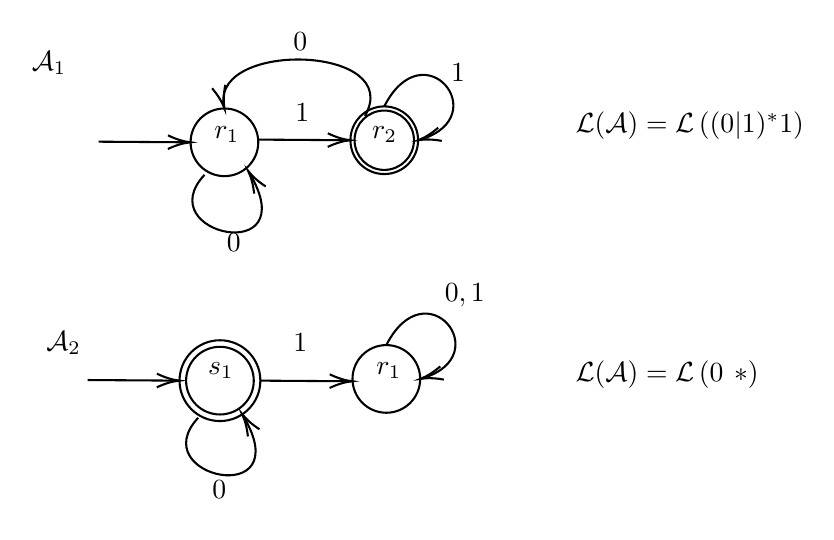
\begin{tikzpicture}[x=0.75pt,y=0.75pt,yscale=-1,xscale=1]
%uncomment if require: \path (0,300); %set diagram left start at 0, and has height of 300

%Shape: Circle [id:dp31987477851432133] 
\draw   (123,57.7) .. controls (123,48.7) and (130.3,41.4) .. (139.3,41.4) .. controls (148.3,41.4) and (155.6,48.7) .. (155.6,57.7) .. controls (155.6,66.7) and (148.3,74) .. (139.3,74) .. controls (130.3,74) and (123,66.7) .. (123,57.7) -- cycle ;
%Straight Lines [id:da966979714088516] 
\draw    (78.67,57.4) -- (121,57.69) ;
\draw [shift={(123,57.7)}, rotate = 180.39] [color={rgb, 255:red, 0; green, 0; blue, 0 }  ][line width=0.75]    (10.93,-3.29) .. controls (6.95,-1.4) and (3.31,-0.3) .. (0,0) .. controls (3.31,0.3) and (6.95,1.4) .. (10.93,3.29)   ;
%Shape: Circle [id:dp7258335773184826] 
\draw   (200,56.7) .. controls (200,47.7) and (207.3,40.4) .. (216.3,40.4) .. controls (225.3,40.4) and (232.6,47.7) .. (232.6,56.7) .. controls (232.6,65.7) and (225.3,73) .. (216.3,73) .. controls (207.3,73) and (200,65.7) .. (200,56.7) -- cycle ;
%Straight Lines [id:da09326584743007293] 
\draw    (155.67,56.4) -- (198,56.69) ;
\draw [shift={(200,56.7)}, rotate = 180.39] [color={rgb, 255:red, 0; green, 0; blue, 0 }  ][line width=0.75]    (10.93,-3.29) .. controls (6.95,-1.4) and (3.31,-0.3) .. (0,0) .. controls (3.31,0.3) and (6.95,1.4) .. (10.93,3.29)   ;
%Curve Lines [id:da8490410391707425] 
\draw    (216.3,40.4) .. controls (235.38,2.97) and (269.62,45.1) .. (234.26,56.21) ;
\draw [shift={(232.6,56.7)}, rotate = 344.86] [color={rgb, 255:red, 0; green, 0; blue, 0 }  ][line width=0.75]    (10.93,-3.29) .. controls (6.95,-1.4) and (3.31,-0.3) .. (0,0) .. controls (3.31,0.3) and (6.95,1.4) .. (10.93,3.29)   ;
%Curve Lines [id:da9263162090026467] 
\draw    (129.67,73.4) .. controls (102.94,102.11) and (178.14,118.08) .. (151.51,72.79) ;
\draw [shift={(150.67,71.4)}, rotate = 58.32] [color={rgb, 255:red, 0; green, 0; blue, 0 }  ][line width=0.75]    (10.93,-3.29) .. controls (6.95,-1.4) and (3.31,-0.3) .. (0,0) .. controls (3.31,0.3) and (6.95,1.4) .. (10.93,3.29)   ;
%Curve Lines [id:da6000311017096592] 
\draw    (207,45) .. controls (226.27,11.09) and (134.46,8.49) .. (138.91,39.46) ;
\draw [shift={(139.3,41.4)}, rotate = 255.34] [color={rgb, 255:red, 0; green, 0; blue, 0 }  ][line width=0.75]    (10.93,-3.29) .. controls (6.95,-1.4) and (3.31,-0.3) .. (0,0) .. controls (3.31,0.3) and (6.95,1.4) .. (10.93,3.29)   ;
%Shape: Circle [id:dp9836812970413046] 
\draw   (202,56.7) .. controls (202,48.8) and (208.4,42.4) .. (216.3,42.4) .. controls (224.2,42.4) and (230.6,48.8) .. (230.6,56.7) .. controls (230.6,64.6) and (224.2,71) .. (216.3,71) .. controls (208.4,71) and (202,64.6) .. (202,56.7) -- cycle ;
%Shape: Circle [id:dp3778621840361358] 
\draw   (117.67,172.53) .. controls (117.67,161.78) and (126.38,153.07) .. (137.13,153.07) .. controls (147.88,153.07) and (156.6,161.78) .. (156.6,172.53) .. controls (156.6,183.28) and (147.88,192) .. (137.13,192) .. controls (126.38,192) and (117.67,183.28) .. (117.67,172.53) -- cycle ;
%Shape: Circle [id:dp8661743582784995] 
\draw   (120.83,172.53) .. controls (120.83,163.53) and (128.13,156.23) .. (137.13,156.23) .. controls (146.14,156.23) and (153.43,163.53) .. (153.43,172.53) .. controls (153.43,181.54) and (146.14,188.83) .. (137.13,188.83) .. controls (128.13,188.83) and (120.83,181.54) .. (120.83,172.53) -- cycle ;
%Straight Lines [id:da5202176824097801] 
\draw    (73.33,172.23) -- (115.67,172.52) ;
\draw [shift={(117.67,172.53)}, rotate = 180.39] [color={rgb, 255:red, 0; green, 0; blue, 0 }  ][line width=0.75]    (10.93,-3.29) .. controls (6.95,-1.4) and (3.31,-0.3) .. (0,0) .. controls (3.31,0.3) and (6.95,1.4) .. (10.93,3.29)   ;
%Straight Lines [id:da010121986176936604] 
\draw    (156.6,172.53) -- (198.93,172.82) ;
\draw [shift={(200.93,172.83)}, rotate = 180.39] [color={rgb, 255:red, 0; green, 0; blue, 0 }  ][line width=0.75]    (10.93,-3.29) .. controls (6.95,-1.4) and (3.31,-0.3) .. (0,0) .. controls (3.31,0.3) and (6.95,1.4) .. (10.93,3.29)   ;
%Shape: Circle [id:dp3268056661855697] 
\draw   (201,171.7) .. controls (201,162.7) and (208.3,155.4) .. (217.3,155.4) .. controls (226.3,155.4) and (233.6,162.7) .. (233.6,171.7) .. controls (233.6,180.7) and (226.3,188) .. (217.3,188) .. controls (208.3,188) and (201,180.7) .. (201,171.7) -- cycle ;
%Curve Lines [id:da5397719576236358] 
\draw    (126.67,190.4) .. controls (99.94,219.11) and (175.14,235.08) .. (148.51,189.79) ;
\draw [shift={(147.67,188.4)}, rotate = 58.32] [color={rgb, 255:red, 0; green, 0; blue, 0 }  ][line width=0.75]    (10.93,-3.29) .. controls (6.95,-1.4) and (3.31,-0.3) .. (0,0) .. controls (3.31,0.3) and (6.95,1.4) .. (10.93,3.29)   ;
%Curve Lines [id:da6138363427217985] 
\draw    (217.3,155.4) .. controls (236.38,117.97) and (270.62,160.1) .. (235.26,171.21) ;
\draw [shift={(233.6,171.7)}, rotate = 344.86] [color={rgb, 255:red, 0; green, 0; blue, 0 }  ][line width=0.75]    (10.93,-3.29) .. controls (6.95,-1.4) and (3.31,-0.3) .. (0,0) .. controls (3.31,0.3) and (6.95,1.4) .. (10.93,3.29)   ;

% Text Node
\draw (45,12.4) node [anchor=north west][inner sep=0.75pt]    {$\mathcal{A}_{1}$};
% Text Node
\draw (52,147.4) node [anchor=north west][inner sep=0.75pt]    {$\mathcal{A}_{2}$};
% Text Node
\draw (247,18.4) node [anchor=north west][inner sep=0.75pt]    {$1$};
% Text Node
\draw (171,3.4) node [anchor=north west][inner sep=0.75pt]    {$0$};
% Text Node
\draw (172,37.4) node [anchor=north west][inner sep=0.75pt]    {$1$};
% Text Node
\draw (139,100.4) node [anchor=north west][inner sep=0.75pt]    {$0$};
% Text Node
\draw (133,48.4) node [anchor=north west][inner sep=0.75pt]    {$r_{1}$};
% Text Node
\draw (209,48.4) node [anchor=north west][inner sep=0.75pt]    {$r_{2}$};
% Text Node
\draw (307,41.4) node [anchor=north west][inner sep=0.75pt]    {$\mathcal{L}(\mathcal{A} ) =\mathcal{L}\left(( 0|1)^{*} 1\right)$};
% Text Node
\draw (130,162.4) node [anchor=north west][inner sep=0.75pt]    {$s_{1}$};
% Text Node
\draw (211,162.4) node [anchor=north west][inner sep=0.75pt]    {$r_{1}$};
% Text Node
\draw (132,219.4) node [anchor=north west][inner sep=0.75pt]    {$0$};
% Text Node
\draw (244,124.4) node [anchor=north west][inner sep=0.75pt]    {$0,1$};
% Text Node
\draw (171,148.4) node [anchor=north west][inner sep=0.75pt]    {$1$};
% Text Node
\draw (307,161.4) node [anchor=north west][inner sep=0.75pt]    {$\mathcal{L}(\mathcal{A}) =\mathcal{L}\left( 0^{\ } *\right)$};


\end{tikzpicture}
\end{center}
\end{exemple}

\begin{proposition}
    Si $\mathcal{A}$ est un NFA, alors il existe un NFA $\mathcal{A}'$ tel que $\mathcal{L}(\mathcal{A}) = \mathcal{L}$ et $\mathcal{L}(\mathcal{A}')= \mathcal{L}^* $.
\end{proposition}

\begin{proof}
    
    Soit $\mathcal{A} = (Q, \Sigma, \delta, q_0, F)$ un NFA. On construit le NFA $\mathcal{A}' = (Q', \Sigma, \delta', q_0', F')$ de la manière suivante :
    \begin{itemize}
        \item $Q' = Q \cup \{q_0'\}$ où $q_0'$ est un nouvel état initial.
        \item $\delta'(q_0', a) = \delta(q_0, a)$ pour tout $a \in \Sigma$ et $\delta'(q_0', \epsilon) = F$.
        \item $\delta'(q, a) = \delta(q, a)$ pour tout $q \in Q$ et $a \in \Sigma$.
        \item $F' = F$.
    \end{itemize}
    Ainsi, $\mathcal{A}'$ accepte toutes les chaînes qui peuvent être obtenues en concaténant zéro ou plusieurs chaînes acceptées par $\mathcal{A}$, ce qui correspond à l'étoile de Kleene de $\mathcal{L}(\mathcal{A})$. Par conséquent, $\mathcal{L}(\mathcal{A}') = \mathcal{L}^*$.
\end{proof}

\begin{exemple}
    Considérons le NFA $\mathcal{A}$ suivant : qui est $\mathcal{L}(\mathcal{A})= \mathcal{L}((a|b)^*bb(\varepsilon | a))$
\end{exemple}

Nous avons $E$ un RegExp on veut à présent construire un NFA $\mathcal{A}$ tel que $\mathcal{L}(\mathcal{A}) = \mathcal{L}(E)$. 
\begin{itemize}
    \item Si $E$ est atomique.
    \begin{itemize}
        \item $E= a$ où $a \in \Sigma$
        \item $E= \varepsilon$
        \item $E= \emptyset$
    \end{itemize}
\end{itemize}
En fait nous avons déjà vu comment construire un NFA pour ces trois cas.

On veut construire un NFA pour $(a|ab)^*$:
\textbf{Atomiques :}
a faire notes
\textbf{Composite :}
à faire voir notes 


DFA -> RegExp


\tikzset{every picture/.style={line width=0.75pt}} %set default line width to 0.75pt        

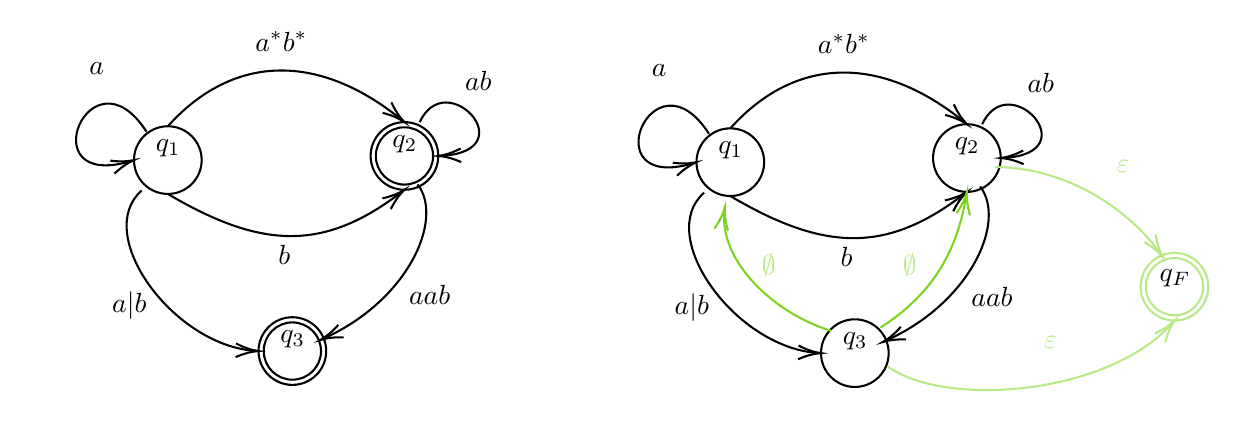
\begin{tikzpicture}[x=0.75pt,y=0.75pt,yscale=-1,xscale=1]
%uncomment if require: \path (0,300); %set diagram left start at 0, and has height of 300

%Shape: Circle [id:dp12668707587199546] 
\draw   (78,106.7) .. controls (78,97.7) and (85.3,90.4) .. (94.3,90.4) .. controls (103.3,90.4) and (110.6,97.7) .. (110.6,106.7) .. controls (110.6,115.7) and (103.3,123) .. (94.3,123) .. controls (85.3,123) and (78,115.7) .. (78,106.7) -- cycle ;
%Shape: Circle [id:dp7829052204770832] 
\draw   (192,104.7) .. controls (192,95.7) and (199.3,88.4) .. (208.3,88.4) .. controls (217.3,88.4) and (224.6,95.7) .. (224.6,104.7) .. controls (224.6,113.7) and (217.3,121) .. (208.3,121) .. controls (199.3,121) and (192,113.7) .. (192,104.7) -- cycle ;
%Curve Lines [id:da044391413322485196] 
\draw    (94.3,90.4) .. controls (126.34,54.76) and (167.83,55.38) .. (207.11,87.42) ;
\draw [shift={(208.3,88.4)}, rotate = 219.78] [color={rgb, 255:red, 0; green, 0; blue, 0 }  ][line width=0.75]    (10.93,-3.29) .. controls (6.95,-1.4) and (3.31,-0.3) .. (0,0) .. controls (3.31,0.3) and (6.95,1.4) .. (10.93,3.29)   ;
%Curve Lines [id:da6459719317875692] 
\draw    (94.3,123) .. controls (140.2,150.13) and (170.07,150.4) .. (207.17,121.87) ;
\draw [shift={(208.3,121)}, rotate = 142] [color={rgb, 255:red, 0; green, 0; blue, 0 }  ][line width=0.75]    (10.93,-3.29) .. controls (6.95,-1.4) and (3.31,-0.3) .. (0,0) .. controls (3.31,0.3) and (6.95,1.4) .. (10.93,3.29)   ;
%Shape: Circle [id:dp37852520087956276] 
\draw   (194.5,104.7) .. controls (194.5,97.08) and (200.68,90.9) .. (208.3,90.9) .. controls (215.92,90.9) and (222.1,97.08) .. (222.1,104.7) .. controls (222.1,112.32) and (215.92,118.5) .. (208.3,118.5) .. controls (200.68,118.5) and (194.5,112.32) .. (194.5,104.7) -- cycle ;
%Curve Lines [id:da21803756035015287] 
\draw    (84,93) .. controls (56.94,50.83) and (27.27,121.95) .. (76.48,107.17) ;
\draw [shift={(78,106.7)}, rotate = 161.98] [color={rgb, 255:red, 0; green, 0; blue, 0 }  ][line width=0.75]    (10.93,-3.29) .. controls (6.95,-1.4) and (3.31,-0.3) .. (0,0) .. controls (3.31,0.3) and (6.95,1.4) .. (10.93,3.29)   ;
%Curve Lines [id:da10179101251687384] 
\draw    (215.67,88.4) .. controls (228.47,60.82) and (266.5,102.13) .. (226.48,104.61) ;
\draw [shift={(224.6,104.7)}, rotate = 358.27] [color={rgb, 255:red, 0; green, 0; blue, 0 }  ][line width=0.75]    (10.93,-3.29) .. controls (6.95,-1.4) and (3.31,-0.3) .. (0,0) .. controls (3.31,0.3) and (6.95,1.4) .. (10.93,3.29)   ;
%Shape: Circle [id:dp03425850462808144] 
\draw   (138,198.7) .. controls (138,189.7) and (145.3,182.4) .. (154.3,182.4) .. controls (163.3,182.4) and (170.6,189.7) .. (170.6,198.7) .. controls (170.6,207.7) and (163.3,215) .. (154.3,215) .. controls (145.3,215) and (138,207.7) .. (138,198.7) -- cycle ;
%Shape: Circle [id:dp8420640618814548] 
\draw   (140.5,198.7) .. controls (140.5,191.08) and (146.68,184.9) .. (154.3,184.9) .. controls (161.92,184.9) and (168.1,191.08) .. (168.1,198.7) .. controls (168.1,206.32) and (161.92,212.5) .. (154.3,212.5) .. controls (146.68,212.5) and (140.5,206.32) .. (140.5,198.7) -- cycle ;
%Curve Lines [id:da23558386270915044] 
\draw    (214.67,118.4) .. controls (227.54,135.23) and (210.02,174.6) .. (168.92,192.85) ;
\draw [shift={(167.67,193.4)}, rotate = 336.8] [color={rgb, 255:red, 0; green, 0; blue, 0 }  ][line width=0.75]    (10.93,-3.29) .. controls (6.95,-1.4) and (3.31,-0.3) .. (0,0) .. controls (3.31,0.3) and (6.95,1.4) .. (10.93,3.29)   ;
%Curve Lines [id:da1528381714909124] 
\draw    (81.67,121.4) .. controls (58.03,142.08) and (96.48,195.76) .. (136.19,198.61) ;
\draw [shift={(138,198.7)}, rotate = 181.85] [color={rgb, 255:red, 0; green, 0; blue, 0 }  ][line width=0.75]    (10.93,-3.29) .. controls (6.95,-1.4) and (3.31,-0.3) .. (0,0) .. controls (3.31,0.3) and (6.95,1.4) .. (10.93,3.29)   ;
%Shape: Circle [id:dp2030319174852412] 
\draw   (349,107.7) .. controls (349,98.7) and (356.3,91.4) .. (365.3,91.4) .. controls (374.3,91.4) and (381.6,98.7) .. (381.6,107.7) .. controls (381.6,116.7) and (374.3,124) .. (365.3,124) .. controls (356.3,124) and (349,116.7) .. (349,107.7) -- cycle ;
%Shape: Circle [id:dp26796860098575603] 
\draw   (463,105.7) .. controls (463,96.7) and (470.3,89.4) .. (479.3,89.4) .. controls (488.3,89.4) and (495.6,96.7) .. (495.6,105.7) .. controls (495.6,114.7) and (488.3,122) .. (479.3,122) .. controls (470.3,122) and (463,114.7) .. (463,105.7) -- cycle ;
%Curve Lines [id:da42556436230102035] 
\draw    (365.3,91.4) .. controls (397.34,55.76) and (438.83,56.38) .. (478.11,88.42) ;
\draw [shift={(479.3,89.4)}, rotate = 219.78] [color={rgb, 255:red, 0; green, 0; blue, 0 }  ][line width=0.75]    (10.93,-3.29) .. controls (6.95,-1.4) and (3.31,-0.3) .. (0,0) .. controls (3.31,0.3) and (6.95,1.4) .. (10.93,3.29)   ;
%Curve Lines [id:da7208114387365273] 
\draw    (365.3,124) .. controls (411.2,151.13) and (441.07,151.4) .. (478.17,122.87) ;
\draw [shift={(479.3,122)}, rotate = 142] [color={rgb, 255:red, 0; green, 0; blue, 0 }  ][line width=0.75]    (10.93,-3.29) .. controls (6.95,-1.4) and (3.31,-0.3) .. (0,0) .. controls (3.31,0.3) and (6.95,1.4) .. (10.93,3.29)   ;
%Curve Lines [id:da5070037541662733] 
\draw    (355,94) .. controls (327.94,51.83) and (298.27,122.95) .. (347.48,108.17) ;
\draw [shift={(349,107.7)}, rotate = 161.98] [color={rgb, 255:red, 0; green, 0; blue, 0 }  ][line width=0.75]    (10.93,-3.29) .. controls (6.95,-1.4) and (3.31,-0.3) .. (0,0) .. controls (3.31,0.3) and (6.95,1.4) .. (10.93,3.29)   ;
%Curve Lines [id:da12401117152167529] 
\draw    (486.67,89.4) .. controls (499.47,61.82) and (537.5,103.13) .. (497.48,105.61) ;
\draw [shift={(495.6,105.7)}, rotate = 358.27] [color={rgb, 255:red, 0; green, 0; blue, 0 }  ][line width=0.75]    (10.93,-3.29) .. controls (6.95,-1.4) and (3.31,-0.3) .. (0,0) .. controls (3.31,0.3) and (6.95,1.4) .. (10.93,3.29)   ;
%Shape: Circle [id:dp8630361797731559] 
\draw   (409,199.7) .. controls (409,190.7) and (416.3,183.4) .. (425.3,183.4) .. controls (434.3,183.4) and (441.6,190.7) .. (441.6,199.7) .. controls (441.6,208.7) and (434.3,216) .. (425.3,216) .. controls (416.3,216) and (409,208.7) .. (409,199.7) -- cycle ;
%Curve Lines [id:da22188124321521796] 
\draw    (485.67,119.4) .. controls (498.54,136.23) and (481.02,175.6) .. (439.92,193.85) ;
\draw [shift={(438.67,194.4)}, rotate = 336.8] [color={rgb, 255:red, 0; green, 0; blue, 0 }  ][line width=0.75]    (10.93,-3.29) .. controls (6.95,-1.4) and (3.31,-0.3) .. (0,0) .. controls (3.31,0.3) and (6.95,1.4) .. (10.93,3.29)   ;
%Curve Lines [id:da03716810781925006] 
\draw    (352.67,122.4) .. controls (329.03,143.08) and (367.48,196.76) .. (407.19,199.61) ;
\draw [shift={(409,199.7)}, rotate = 181.85] [color={rgb, 255:red, 0; green, 0; blue, 0 }  ][line width=0.75]    (10.93,-3.29) .. controls (6.95,-1.4) and (3.31,-0.3) .. (0,0) .. controls (3.31,0.3) and (6.95,1.4) .. (10.93,3.29)   ;
%Curve Lines [id:da24561821068886103] 
\draw [color={rgb, 255:red, 184; green, 233; blue, 134 }  ,draw opacity=1 ]   (493,110) .. controls (527.95,110.39) and (557.46,130.57) .. (572.75,152.08) ;
\draw [shift={(573.67,153.4)}, rotate = 235.71] [color={rgb, 255:red, 184; green, 233; blue, 134 }  ,draw opacity=1 ][line width=0.75]    (10.93,-3.29) .. controls (6.95,-1.4) and (3.31,-0.3) .. (0,0) .. controls (3.31,0.3) and (6.95,1.4) .. (10.93,3.29)   ;
%Curve Lines [id:da03371338051788353] 
\draw [color={rgb, 255:red, 184; green, 233; blue, 134 }  ,draw opacity=1 ]   (441,206) .. controls (468.39,226.2) and (547.69,220.13) .. (578.38,185.07) ;
\draw [shift={(579.3,184)}, rotate = 129.81] [color={rgb, 255:red, 184; green, 233; blue, 134 }  ,draw opacity=1 ][line width=0.75]    (10.93,-3.29) .. controls (6.95,-1.4) and (3.31,-0.3) .. (0,0) .. controls (3.31,0.3) and (6.95,1.4) .. (10.93,3.29)   ;
%Shape: Circle [id:dp9266974895346719] 
\draw  [color={rgb, 255:red, 184; green, 233; blue, 134 }  ,draw opacity=1 ] (563,167.7) .. controls (563,158.7) and (570.3,151.4) .. (579.3,151.4) .. controls (588.3,151.4) and (595.6,158.7) .. (595.6,167.7) .. controls (595.6,176.7) and (588.3,184) .. (579.3,184) .. controls (570.3,184) and (563,176.7) .. (563,167.7) -- cycle ;
%Shape: Circle [id:dp9338220019696463] 
\draw  [color={rgb, 255:red, 184; green, 233; blue, 134 }  ,draw opacity=1 ] (565.5,167.7) .. controls (565.5,160.08) and (571.68,153.9) .. (579.3,153.9) .. controls (586.92,153.9) and (593.1,160.08) .. (593.1,167.7) .. controls (593.1,175.32) and (586.92,181.5) .. (579.3,181.5) .. controls (571.68,181.5) and (565.5,175.32) .. (565.5,167.7) -- cycle ;
%Curve Lines [id:da34354886386764727] 
\draw [color={rgb, 255:red, 126; green, 211; blue, 33 }  ,draw opacity=1 ]   (414,189) .. controls (386.38,180.61) and (360.02,155.69) .. (362.42,131.28) ;
\draw [shift={(362.67,129.4)}, rotate = 99.09] [color={rgb, 255:red, 126; green, 211; blue, 33 }  ,draw opacity=1 ][line width=0.75]    (10.93,-3.29) .. controls (6.95,-1.4) and (3.31,-0.3) .. (0,0) .. controls (3.31,0.3) and (6.95,1.4) .. (10.93,3.29)   ;
%Curve Lines [id:da4300413384622155] 
\draw [color={rgb, 255:red, 126; green, 211; blue, 33 }  ,draw opacity=1 ]   (437.67,187.4) .. controls (464.97,169.85) and (474.81,148.12) .. (478.99,123.87) ;
\draw [shift={(479.3,122)}, rotate = 99.09] [color={rgb, 255:red, 126; green, 211; blue, 33 }  ,draw opacity=1 ][line width=0.75]    (10.93,-3.29) .. controls (6.95,-1.4) and (3.31,-0.3) .. (0,0) .. controls (3.31,0.3) and (6.95,1.4) .. (10.93,3.29)   ;

% Text Node
\draw (87,95.4) node [anchor=north west][inner sep=0.75pt]    {$q_{1}$};
% Text Node
\draw (201,93.4) node [anchor=north west][inner sep=0.75pt]    {$q_{2}$};
% Text Node
\draw (147,187.4) node [anchor=north west][inner sep=0.75pt]    {$q_{3}$};
% Text Node
\draw (135,43.4) node [anchor=north west][inner sep=0.75pt]    {$a^{*} b^{*}$};
% Text Node
\draw (146,146.4) node [anchor=north west][inner sep=0.75pt]    {$b$};
% Text Node
\draw (236,62.4) node [anchor=north west][inner sep=0.75pt]    {$ab$};
% Text Node
\draw (209,165.4) node [anchor=north west][inner sep=0.75pt]    {$aab$};
% Text Node
\draw (66,168.4) node [anchor=north west][inner sep=0.75pt]    {$a|b$};
% Text Node
\draw (55,58.4) node [anchor=north west][inner sep=0.75pt]    {$a$};
% Text Node
\draw (358,96.4) node [anchor=north west][inner sep=0.75pt]    {$q_{1}$};
% Text Node
\draw (472,94.4) node [anchor=north west][inner sep=0.75pt]    {$q_{2}$};
% Text Node
\draw (418,188.4) node [anchor=north west][inner sep=0.75pt]    {$q_{3}$};
% Text Node
\draw (406,44.4) node [anchor=north west][inner sep=0.75pt]    {$a^{*} b^{*}$};
% Text Node
\draw (417,147.4) node [anchor=north west][inner sep=0.75pt]    {$b$};
% Text Node
\draw (507,63.4) node [anchor=north west][inner sep=0.75pt]    {$ab$};
% Text Node
\draw (480,166.4) node [anchor=north west][inner sep=0.75pt]    {$aab$};
% Text Node
\draw (337,169.4) node [anchor=north west][inner sep=0.75pt]    {$a|b$};
% Text Node
\draw (326,59.4) node [anchor=north west][inner sep=0.75pt]    {$a$};
% Text Node
\draw (570.67,157.8) node [anchor=north west][inner sep=0.75pt]    {$q_{F}$};
% Text Node
\draw (550,105.4) node [anchor=north west][inner sep=0.75pt]  [color={rgb, 255:red, 184; green, 233; blue, 134 }  ,opacity=1 ]  {$\varepsilon $};
% Text Node
\draw (515,190.4) node [anchor=north west][inner sep=0.75pt]  [color={rgb, 255:red, 184; green, 233; blue, 134 }  ,opacity=1 ]  {$\varepsilon $};
% Text Node
\draw (379,150.4) node [anchor=north west][inner sep=0.75pt]  [color={rgb, 255:red, 184; green, 233; blue, 134 }  ,opacity=1 ]  {$\emptyset $};
% Text Node
\draw (447,150.4) node [anchor=north west][inner sep=0.75pt]  [color={rgb, 255:red, 184; green, 233; blue, 134 }  ,opacity=1 ]  {$\emptyset $};


\end{tikzpicture}

Soit $\mathcal{A}=(Q, \Sigma, \delta, q_0, F)$ un automate en forme spéciale. 

*avant ça à retravailler sur les notes c'est un peu brouillon*

%====================================================================
\section*{V. Forme canonique et minimisation}
%====================================================================

Nous avons vu que les expressions régulières (RegExp) n'ont pas de forme canonique, ce qui rend leur comparaison difficile.

Mais, grâce au théorème de Kleene, nous savons qu'une RegExp n'est qu'une des représentations possibles d'un langage régulier : nous avons aussi accès aux automates. Nous allons voir que \emph{ces derniers admettent une forme canonique}. Ils seront donc à privilégier pour comparer (et, plus généralement, manipuler) des langages.

\paragraph{Idée.}
Pour un langage $\mathcal{L}$, on va classer les mots $w \in \Sigma^*$ en fonction des continuations possibles et de leur impact sur l'appartenance à $\mathcal{L}$. Deux mots $w_1$ et $w_2$ qui sont équivalents vis-à-vis des continuations seront dans la même classe.

\begin{quote}
\small\itshape
Anil Nerode (1932--), logicien américain : logique, langages, complexité, etc.
\end{quote}

\begin{definition}[Congruence de Nerode]
Pour un mot $w \in \Sigma^*$ et un langage $\mathcal{L} \subseteq \Sigma^*$, on définit
\[
w^{-1}\mathcal{L} = \{\, w' \in \Sigma^* \mid ww' \in \mathcal{L} \,\},
\]
l'ensemble des continuations $w'$ de $w$ telles que $ww' \in \mathcal{L}$.

On définit la relation d'équivalence ${\sim_{\mathcal{L}}} \subseteq \Sigma^* \times \Sigma^*$ par
\[
w_1 \sim_{\mathcal{L}} w_2 \iff w_1^{-1}\mathcal{L} = w_2^{-1}\mathcal{L}.
\]
\end{definition}

% (Un exemple suivait au tableau : à compléter.)

On va en tirer une caractérisation de l'automate \emph{minimal} pour un langage $\mathcal{L}$. C'est important quand on utilise les automates comme structure de données.

\begin{quote}
\small\itshape
John Myhill (1923--1987), mathématicien anglais. Pionnier en théorie des langages, théorie des ensembles, calculabilité, etc.
\end{quote}

\begin{theoreme}[Myhill--Nerode]
\leavevmode
\begin{enumerate}
  \item Un langage $\mathcal{L}$ est régulier ssi $\sim_{\mathcal{L}}$ a un nombre fini de classes d'équivalence.
  \item Ce nombre est égal au nombre minimal d'états d'un DFA reconnaissant $\mathcal{L}$.
  \item Ce DFA minimal est unique à isomorphisme près.
\end{enumerate}
\end{theoreme}

\begin{remarque}
On obtient ainsi une \emph{troisième caractérisation} de la régularité d'un langage.
\end{remarque}

\begin{exemple}
Considérons l'automate $\mathcal{A}$ suivant :
\begin{center}
\begin{tikzpicture}[shorten >=1pt, node distance=2.2cm, on grid, auto, >={Stealth}]
  \node[state, initial, initial text={}] (q1) {$q_1$};
  \node[state] (q2) [right=of q1] {$q_2$};
  \node[state] (q3) [right=of q2] {$q_3$};
  \node[state, accepting] (q4) [right=of q3] {$q_4$};
  \path[->]
    (q1) edge [loop above] node {$0$} ()
         edge node {$1$} (q2)
    (q2) edge [loop above] node {$1$} ()
         edge node {$0$} (q3)
    (q3) edge [bend left=40] node {$0$} (q1)
         edge node {$1$} (q4)
    (q4) edge [loop above] node {$0,1$} ();
\end{tikzpicture}
\end{center}
Notre automate pour $(0|1)^*\,101\,(0|1)^*$ est-il minimal ?

Considérons
\[
w_1 = \varepsilon, \qquad w_2 = 1, \qquad w_3 = 10, \qquad w_4 = 101.
\]
Chaque $w_i$ est celui qui nous a inspiré pour créer $q_i$. On a bien $w_i \not\sim_{\mathcal{L}} w_j$ pour tout $i \neq j$ :
\begin{itemize}
  \item $w_1 \not\sim_{\mathcal{L}} w_2$ car $w_1 01 \notin \mathcal{L}$ et $w_2 01 \in \mathcal{L}$ ;
  \item $w_2 \not\sim_{\mathcal{L}} w_3$ car $w_2 1 \notin \mathcal{L}$ et $w_3 1 \in \mathcal{L}$ ;
  \item $w_3 \not\sim_{\mathcal{L}} w_4$ car $w_3 \varepsilon \notin \mathcal{L}$ et $w_4 \varepsilon \in \mathcal{L}$ ;
  \item $w_1 \not\sim_{\mathcal{L}} w_3$ car $w_1 1 \notin \mathcal{L}$ et $w_3 1 \in \mathcal{L}$ ;
  \item $w_1 \not\sim_{\mathcal{L}} w_4$ car $w_1 \varepsilon \notin \mathcal{L}$ et $w_4 \varepsilon \in \mathcal{L}$ ;
  \item $w_2 \not\sim_{\mathcal{L}} w_4$ car $w_2 \varepsilon \notin \mathcal{L}$ et $w_4 \varepsilon \in \mathcal{L}$.
\end{itemize}
Nous avions donc déjà l'automate minimal.
\end{exemple}

\begin{remarque}
Les états de l'automate minimal correspondent aux classes de $\sim_{\mathcal{L}}$.
L'existence d'un automate minimal (à isomorphisme près) est intéressante, mais on voudrait aussi pouvoir le calculer.
\end{remarque}

\subsection*{Minimisation de DFA}

\begin{proposition}
Étant donné un DFA $\mathcal{A}$, on peut construire un DFA minimal $\mathcal{A}'$ tel que $\mathcal{L}(\mathcal{A}') = \mathcal{L}(\mathcal{A})$ en \emph{temps polynomial}.
\end{proposition}

\begin{remarque}
Cela deviendra plus clair dans le chapitre « Complexité », mais c'est une bonne nouvelle.
On ne verra pas l'algorithme ; allez voir Esparza et Blondin si cela vous intéresse.
\end{remarque}

\subsection*{Quid des NFA ?}

Malheureusement, il n'y a pas d'unicité de l'automate minimal. Considérons $\mathcal{L} = \mathcal{L}(aa^*)$.
\begin{center}
\begin{tikzpicture}[shorten >=1pt, node distance=2cm, on grid, auto, >={Stealth}]
  \node at (-1.2,0) {$\mathcal{A}_1$};
  \node[state, initial, initial text={}] (p0) at (0,0) {};
  \node[state, accepting] (p1) [right=of p0] {};
  \path[->]
    (p0) edge node {$a$} (p1)
    (p1) edge [loop above] node {$a$} ();

  \node at (5.3,0) {$\mathcal{A}_2$};
  \node[state, initial, initial text={}] (r0) at (6.5,0) {};
  \node[state, accepting] (r1) [right=of r0] {};
  \path[->]
    (r0) edge [loop above] node {$a$} ()
         edge node {$a$} (r1);
\end{tikzpicture}
\end{center}
Nous avons deux automates minimaux qui ne sont pas isomorphes ! Cela rend les choses beaucoup plus compliquées.

\begin{theoreme}[Complexité de la minimisation de NFA]
Soient $\mathcal{A}$ un NFA et $k \geq 1$. Décider s'il existe un NFA $\mathcal{A}'$ avec au plus $k$ états tel que $\mathcal{L}(\mathcal{A}') = \mathcal{L}(\mathcal{A})$ est un problème \emph{PSPACE-complet}.
\end{theoreme}

\begin{remarque}
Ça, par contre, c'est une mauvaise nouvelle ! En pratique, cela demande un temps exponentiel ; on ne sait pas si un algorithme polynomial existe (et on pense que non, sinon $\mathrm{P} = \mathrm{PSPACE}$).
\end{remarque}

%====================================================================
\section*{VI. Caractérisation logique}
%====================================================================

Pour faire le lien avec IntLog, considérons une dernière caractérisation des langages réguliers, via la logique. Il existe deux philosophies de description des langages :

\begin{center}
\begin{tabular}{p{0.42\textwidth}|p{0.42\textwidth}}
\multicolumn{1}{c|}{\textbf{RegExp}} & \multicolumn{1}{c}{\textbf{Logique}} \\
\hline
Description \emph{générationnelle} : « comment créer un mot du langage ». &
Description \emph{déclarative} : « propriété à satisfaire pour appartenir au langage ». \\
\end{tabular}
\end{center}

En fonction du langage, l'une ou l'autre description peut être plus facile à comprendre.

\begin{exemple}
Le langage des mots ayant un nombre pair de $a$ et un nombre pair de $b$ :
\[
\mathcal{L} = \{\, w \in \{a,b\}^* \mid \#a \bmod 2 = 0 \ \wedge\ \#b \bmod 2 = 0 \,\}
\]
versus
\[
\mathcal{L}\Big( \big[\, aa \mid bb \mid (ab \mid ba)(aa \mid bb)^*(ba \mid ab) \,\big]^* \Big).
\]
\end{exemple}

Nous allons utiliser la \emph{logique des prédicats sur les mots}, qui est la logique du \emph{premier ordre} : les quantificateurs ne portent que sur les « variables d'individus », jamais sur des propriétés, des prédicats ou des fonctions.

Fixons un alphabet $\Sigma = \{a, b\}$. On distingue deux types de propriétés atomiques :
\begin{enumerate}
  \item $P_a(x)$ ou $P_b(x)$, où $x$ est une variable désignant une position au sein du mot.
  Par exemple, $P_b(7)$ est le prédicat qui est vrai si la lettre à la $7^{\text{e}}$ position est « $b$ ».
  \item $x < y$, où $x$ et $y$ sont deux variables de position.
\end{enumerate}

\begin{exemple}
$\mathcal{L}(a^*b^*)$ : si on a un « $b$ » dans une position, alors on en a aussi dans toutes les suivantes.
En logique des prédicats :
\[
\forall x\, \forall y\, \big[\, (P_b(x) \wedge x < y) \rightarrow P_b(y) \,\big].
\]
\end{exemple}

\begin{exemple}
\[
\forall x\, \forall y\, \Big[\, \big(P_a(x) \wedge x < y \wedge P_a(y)\big) \rightarrow \exists z\, \big(x < z \wedge z < y \wedge P_b(z)\big) \Big]
\]
signifie : entre deux « $a$ », il y a au moins un « $b$ ».
\end{exemple}
